\documentclass[10pt, openany]{book}
\usepackage[FINAL]{../boilerplate/rexx} 
\usepackage{hyperref}
\usepackage{graphics}
\usepackage{fontspec}
% \fontspec
%      [ Path = /Users/rvjansen/Fonts/,
%        BoldFont       = MinionPro-Bold.otf ,
%        ItalicFont     = MinionPro-It.otf ,
%        BoldItalicFont = MinionPro-BoldIt.otf ]
%      {MinionPro-Regular.otf}
% \fontspec
%      [ Path = /Users/rvjansen/Fonts/,
%        BoldFont       = SourceCodePro-Bold.otf ]
%      {SoureCodePro-Regular.otf}

\setmainfont[Mapping=tex-text]{Minion Pro}
\setmonofont[Mapping=tex-text,Scale=0.80]{Source Code Pro}
\usepackage{tabularx}
\usepackage{booktabs}
\usepackage{makeidx}
\usepackage[all]{xy}
%\usepackage{lingmacros}
\usepackage{color}
\usepackage{xcolor}
\usepackage{listings}
\usepackage{caption}
\usepackage{longtable}
\usepackage{colortbl}
\usepackage{framed}
\usepackage{fancyvrb}
\definecolor{shadecolor}{rgb}{0.9,0.9,0.9}
\usepackage{alltt}
\DeclareCaptionFont{white}{\color{white}}
\DeclareCaptionFormat{listing}{\colorbox{gray}{\parbox{\textwidth}{#1#2#3}}}
\captionsetup[lstlisting]{format=listing,labelfont=white,textfont=white}
\usepackage{listings}
\usepackage[official]{eurosym}
\makeatletter
\lst@CCPutMacro\lst@ProcessOther {"2D}{\lst@ttfamily{-{}}{-{}}}
\@empty\z@\@empty
\makeatother
\lstdefinelanguage{NetRexx}
{morekeywords={abstract,adapter,binary,case,catch,class,constant,dependent,deprecated,digits,do,else,end,engineering,extends,final,finally,for,forever,if,implements,indirect,import,indirect,inheritable,interface,iterate,label,leave,loop,method,native,nop,numeric,options,otherwise,over,package,parent,parse,private,properties,protect,public,return,returns,rexx,say,scientific,set,digits,form,select,shared,signal,signals,sourceline,static,super,then,this,until,used,upper,volatile,when,where,while},
sensitive=false,
extendedchars=false,
morecomment=[s]={/*}{*/},
morecomment=[l]{--},
morecomment=[s]{/**}{*/},
morestring=[b]",
morestring=[d]",
morestring=[b]',
morestring=[d]'}

\lstset{language=NetRexx,
  captionpos=t,
  tabsize=3,
  alsolanguage=Rexx,
  keywordstyle=\color{blue},
  commentstyle=\color{cyan},
  stringstyle=\color{red},
  numbers=left,
  numberstyle=\tiny,
  numbersep=5pt,
  breaklines=true,
  showstringspaces=false,
  index=[1][keywords],
  columns=flexible,
  basicstyle=\fontsize{8}{8}\fontspec{Source Code Pro},emph={label}}

\usepackage{../boilerplate/rail}
\usepackage{pst-barcode,pstricks-add}
\usepackage{bashful}
\usepackage{metalogo}
\usepackage{marginnote}
\usepackage{pdfpages}
\usepackage{float}
\hyphenation{Net-Rexx Net-Rexx-A Net-Rexx-C Net-Rexx-R Mac-OSX
  infra-structure im-ple-men-ta-tion-de-pen-dent}
\makeindex
\DeclareGraphicsExtensions{.jpg,.png}
\setlength{\parskip}{4pt}
\setlength{\parindent}{0pt}
\usepackage{enumitem}
\newcommand{\nr}{Net\textsc{Rexx}}
\newcommand{\Rexx}{R\textsc{exx}}
\newcommand{\nrpackagename}{\splice{java GetPackageName}}
\newcommand{\minimalJVMversion}{1.6}
\newcommand{\keyword}[1]{\texttt{#1}}
\newcommand{\code}[1]{\texttt{#1}}
\newcommand{\thisyear}{\splice{java TexYear}}
\newcommand{\ecjjarname}{ecj-4.6.3.jar}
\newcommand{\msd}[1]{\msdhelper#1\relax}
\newcommand{\msdhelper}[1]
  {\ifx\relax#1\else
    \ifx-#1--{}\else#1\fi
    \expandafter\msdhelper\fi}
  \newcommand{\doublehyphen}{\mbox{\msd{``-~-''}}}
  \newcommand{\doublehyphenunquoted}{\mbox{\msd{-~-}}}
%%% Local Variables: 
%%% mode: latex
%%% TeX-master: t
%%% End: 

\begin{document} 
\renewcommand{\isbn}{978-90-819090-0-6}
\setcounter{tocdepth}{1}
\title{\fontspec{Bodoni URW Light}NetR\fontspec{Minion Pro}\textsc{exx}\protect\\\fontspec{Bodoni URW Light}Programming Guide}  
\author{RexxLA}
\date{\null\hfill Version \splice{java org.netrexx.process.NrVersion} of \today}
\maketitle
\pagenumbering{Roman}
\pagestyle{plain}
\frontmatter
\pagenumbering{Roman}
\pagestyle{plain}
\section*{Publication Data}
\textcopyright  Copyright The Rexx Language Association, 2011-\splice{java TexYear}
%\\

All original material in this publication is published under the Creative Commons - Share Alike 3.0 License as stated at \url{http://creativecommons.org/licenses/by-nc-sa/3.0/us/legalcode}.\\[0.5cm]
The responsible publisher of this edition is identified as \emph{IBizz IT Services and Consultancy}, Amsteldijk 14, 1074 HR Amsterdam, a registered company governed by the laws of the Kingdom of The Netherlands.\\[1cm]
This edition is registered under ISBN \isbn \\[1cm]
\psset{unit=1in}
\begin{pspicture}(3.5,1in)
  \psbarcode{\isbn}{includetext guardwhitespace}{isbn}
\end{pspicture}
\newpage
%%% Local Variables:
%%% mode: latex
%%% TeX-master: t
%%% End:

\tableofcontents
\newpage
\pagenumbering{arabic}
\frontmatter
\large
\chapter*{\fontspec{IBM Plex Serif}\LARGE The \nr{} Programming Series}
This book is part of a library, the \emph{\nr{} Programming Series}, documenting the \nr{} programming language and its use and applications. This section lists the other publications in this series, and their roles. These books can be ordered in convenient hardcopy and electronic formats from the Rexx Language Association.
\newline
\newline
\begin{tabularx}{\textwidth}{>{\bfseries}lX}
\toprule
%% Quick Start Guide & This guide is meant for an audience that has done some programming and wants to start quickly. It starts with a quick tour of the language, and a section on installing the \nr{} translator and how to run it. It also contains help for troubleshooting if anything in the installation does not work as designed, and states current limits and restrictions of the open source reference implementation.
%% \\\midrule
Programming Guide & The Programming Guide is the one manual that at the same time teaches programming, shows lots of examples as they occur in the real world, and explains about the internals of the translator and how to interface with it.
\\\midrule
Language Reference & Referred to as the NRL, this is meant as the formal definition for the language, documenting its syntax and semantics, and prescribing minimal functionality for language implementers.
\\\midrule
Pipelines Guide \& Reference & The Data Flow oriented companion to \nr{}, with its CMS Pipelines compatible syntax, is documented in this manual. It discusses running Pipes for \nr{} in the command shell and the Workspace, and has ample examples of defining your own stages in \nr{}.
\\\bottomrule
\end{tabularx}
%%% Local Variables: 
%%% mode: latex
%%% TeX-master: t
%%% End: 

\chapter{Typographical conventions}
In general, the following conventions have  been observed in the NetRexx publications:
\begin{itemize}
\item Body text is in this font
\item Examples of language statements are in a \textbf{bold} type
\item Variables or strings as mentioned in source code, or things that appear on the console, are in a \texttt{typewriter} type
\item Items that are introduced, or emphasized, are in an \emph{italic} type
\item Included program fragments are listed in this fashion:
\begin{lstlisting}[label=example,caption=Example Listing]
-- salute the reader
say 'lectorem salutat'
\end{lstlisting}
\item Syntax diagrams take the form of so-called \emph{Railroad Diagrams} to convey structure, mandatory and optional items
\begin{rail}
AggregateExpression : ("AVG" |"MAX" |"MIN" |"SUM")
 (
   (
    'DISTINCT' ?  StateFieldPathExpression
   ) | 'COUNT'
   (
    'DISTINCT' ?  IdentificationVariable
                  | StateFieldPathExpression
                  | SingleValuedAssociationPathExpression
   )
 )
   ;
\end{rail}
%%% Local Variables: 
%%% mode: latex
%%% TeX-master: t
%%% End: 
\end{itemize}
\chapter{Introduction}
This document is the \emph{Quick Start Guide} for the reference implementation of
\nr{}. \nr{} is a \emph{human-oriented} programming language which makes
writing and using Java\footnote{Java is a trademark of Oracle, Inc.}
classes quicker and easier than writing in Java. It is part of the Rexx
language family, under the governance of the Rexx Language
Association.\footnote{\url{http.www.rexxla.org}} \nr{} has been
developed and was made available as a free download by IBM since 1995
and is free and open source since June 8, 2011.

In this Quick Start Guide, you’ll find information on
\begin{enumerate} 
\item How easy it is to write for the JVM: A Quick Tour of \nr{}
\item Installing \nr{} 
\item Using the \nr{} translator as a compiler, interpreter, or
  syntax checker 
\item Troubleshooting when things do not work as expected
\item Current restrictions.
\end{enumerate} 
The \nr{} documentation and software are distributed
by The Rexx Language Association under the \textsc{ICU} license. For
the terms of this license, see the included \textsc{LICENSE} file in
this package.

For details of the \nr{} language, and the latest news, downloads,
etc., please see the \nr{} documentation included with the package
or available at: \url{http://www.netrexx.org}.

\begin{shaded}\noindent
The highest Java version that is supported in this version, 3.09, is
\emph{Java 8}. Higher versions are not yet supported due to changes in
Java, including incompatibilities introduced with the Java module system.
\end{shaded}\indent

\mainmatter
\chapter{Meet the \Rexx{} Family}
\section{Once upon a Virtual Machine}
On the 22nd of March 1979, to be precise, Mike Cowlishaw of IBM had a
vision of an easier to use command processor for VM, and wrote down a
specification over the following days.
VM\textsuperscript{\texttrademark} (now called z/VM) is the original Virtual Machine operating system,  stemming from an
era in which time sharing was acknowledged to be the wave of the
future and when systems as CTSS (on the IBM 704) and TSS (on the IBM
360 Family of computers) were early timesharing systems, that offered
the user an illusion of having a large machine for their exclusive
use, but fell short of virtualising the entire hardware. The CP/CMS
system changed this; CP virtualised the hardware completely and CMS was the OS
running on CP. CMS knew a succession of command interpreters, called
EXEC, EXEC2 and \Rexx{}\textsuperscript{\texttrademark}  (originally REX
- until it was found out, by the IBM legal department, that a product of another vendor had a similar name) -
the EXEC roots are the explanation why some people refer to a \nr{}
program as an ``exec''. As a prime example of a \emph{backronym}, Rexx
stands for ``Restructured Extended Executor''. It
can be defended that \Rexx{} came to be as a reaction on EXEC2, but it
must be noted that both command interpreters shipped around the same
time. From 1988 on \Rexx{} was available on MVS/TSO and other systems,
like DOS, Amiga and various Unix systems. \Rexx{} was branded the
official SAA procedures language and was implemented on all IBM's
Operating Systems; most people got to know \Rexx{} on OS/2. In the late
eighties the Object-Oriented successor of Rexx, Object Rexx, was
designed by Simon Nash and his colleagues in the IBM Winchester
laboratory. \Rexx{} was thereafter known as Classic Rexx. Several open
source versions of Classic \Rexx{} were made over the years, of which
Regina is a good example.

\section{Once upon another Virtual Machine}
In 1995 Mike Cowlishaw ported Java\textsuperscript{\texttrademark} to OS/2\textsuperscript{\texttrademark} and soon after started with
an experiment to run \Rexx{} on the JVM\textsuperscript{\texttrademark}. With \Rexx{} generally considered
the first of the general purpose scripting languages, \nr{}\textsuperscript{\texttrademark}  is the
first alternative language for the JVM. The 0.50 release, from April
1996, contained the \nr{} runtime classes and a translator written
in \Rexx{} but tokenized and turned into an OS/2 executable. The 1.00
release came available in January 1997 and contained a translator
bootstrapped to \nr{}. The \Rexx{} string type that can also handle
unlimited precision numerics is called \Rexx{} in Java and \nr{}.
Where Classic \Rexx{} was positioned as a system \emph{glue} language and
application macro language, \nr{} is seen as the one language that
does it all, delivering system level programs or large applications.

Release 2.00 became available in August 2000 and was a major upgrade,
in which interpreted execution was added. Until that release, \nr{}
only knew \emph{ahead of time} compilation (AOT).

Mike Cowlishaw took early retirement from IBM in March 2010. IBM
announced the transfer of \nr{{} source code to the \Rexx{} Language
  Association (RexxLA) on June 8, 2011, 14 years after the v1.0
  release, and on the same day, it released the \nr{} source code to RexxLA
under the ICU open source license. RexxLA shortly after released this
as \nr{} 3.00 and has followed with updates.
\section{Features of \nr}
\begin{description}
\item[Ease of use]
The \nr{} language is easy to read and write because many instructions
are meaningful English words. Unlike some lower level programming
languages that use abbreviations, \nr{} instructions are common words, such as \textbf{say}, \textbf{ask}, \textbf{if...then...else}, \textbf{do...end}, and \textbf{exit}.
\item[Free format] There are few rules about \nr{} format. You need not start an instruction in a particular column, you can also skip spaces in a line or skip entire lines, you can have an instruction span many lines or have multiple instructions on one line, variables do not need to be pre-defined, and you can type instructions in upper, lower, or mixed case.
\item[Convenient built-in functions] \nr{} supplies built-in functions
  that perform various processing, searching, and comparison
  operations for both text and numbers. Other built-in functions
  provide formatting capabilities and arithmetic calculations.
\item[Easy to debug]
When a \nr{} exec contains an error, messages with meaningful explanations are displayed on the screen. In addition, the \textbf{trace} instruction provides a powerful debugging tool.
\item[Interpreted]
The \nr{} language is an interpreted language. When a \nr{} exec
runs, the language processor directly interprets each language
statement, or translates the program in JVM bytecode.
\item[Extensive parsing capabilities]
\nr{} includes extensive parsing capabilities for character
manipulation. This parsing capability allows you to set up a pattern
to separate characters, numbers, and mixed input.
\item[Seamless use of JVM Class Libraries]
\nr{} can use any class, and class library for the JVM (written in
Java or other JVM languages) in a seamless manner, that is, without
the need for extra declarations or definitions in the source code.
\end{description}


\chapter{Learning to program}
\section{Console Based Programs}
One way that a computer can communicate with a user is to ask
questions and then compute results based on the answers typed in. In
other words, the user has a conversation with the computer. You can
easily write a list of  \nr{} instructions that will conduct a conversation. We call such a list of instructions a program.
The following listing shows a sample \nr{} program. The sample program asks the user to give his name, and then responds to him by name. For instance, if the user types in the name Joe, the reply Hello Joe is displayed. Or else, if the user does not type anything in, the reply Hello stranger is displayed.
First, we shall discuss how it works; then you can try it out for
yourself.
\begin{lstlisting}[label=hello,caption=Hello Stranger]
/* A conversation */
say "Hello! What's your name?"
who=ask
if who = '' then say "Hello stranger"
else say "Hello" who
\end{lstlisting}
Briefly, the various pieces of the sample program are:
\begin{description}
\item[\texttt{/* ... */}] A comment explaining what the program is
  about. Where \Rexx{} programs on several platforms must start with a comment, this is not
  a hard requirement for \nr{} anymore. Still, it is a good idea to start
  every program with a comment that explains what it does.
\item [\texttt{say}] An instruction to display Hello! What' s your name? on the screen.
\item [\texttt{ask}] An instruction to read the response entered from the keyboard and put it into the computer's memory.
\item [\texttt{who}] The name given to the place in memory where the user's response is put.
\item [\texttt{if}] An instruction that asks a question. 
\item [\texttt{who = ''}] A test to determine if who is empty.
\item [\texttt{then}] A direction to execute the instruction that follows, if the tested condition is true.
\item [\texttt{say}] An instruction to display Hello stranger on the screen.
\item [\texttt{else}] An alternative direction to execute the
  instruction that follows, if the tested condition is not true. Note
  that in \nr{}, else needs to be on a separate line.
\item [\texttt{say}] An instruction to display Hello, followed by whatever is in who on the screen.
\end{description}
The text of your program should be stored on a disk that you have
access to with the help of an \emph{editor} program. On Windows,
notepad or (notepad++), jEdit, X2 or SlickEdit are suitable
candidates. On Unix based systems, including macOS, vim or emacs are
plausible editors. If you are on z/VM or z/OS, XEDIT or ISPF/PDF are a
given. More about editing \nr{} code in chapter \ref{editors},
\emph{Editor Support}, on page \pageref{editors}. 

When the text of the program is stored in a file, let's say we called
it \texttt{hello.nrx}, and you installed \nr{} as indicated in the
\emph{\nr{} QuickStart Guide}, we can run it with
\begin{verbatim}
    nrc -exec hello
\end{verbatim}
and this will yield the result:
\begin{alltt}
\nr{} portable processor, version \nr{} after3.01, build 1-20120406-1326
Copyright (c) RexxLA, 2011.  All rights reserved.
Parts Copyright (c) IBM Corporation, 1995,2008.
Program hello.nrx
===== Exec: hello =====
Hello! What’s your name?
\end{alltt}
If you do not want to see the version and copyright message every
time, which would be understandable, then start the program with:
\begin{verbatim}
nrc -exec -nologo hello
\end{verbatim}
This is what happened when Fred tried it.
\begin{verbatim}
Program hello.nrx
===== Exec: hello =====
Hello! What’s your name?
Fred
Hello Fred
\end{verbatim}
The \textbf{ask} instruction paused, waiting for a reply. Fred typed
Fred on the command line and, when he pressed the ENTER key, the
\textbf{ask} instruction put the word Fred into the place in the
computer's memory called ``who''. The \textbf{if} instruction asked,
is ``who'' equal to nothing:
\begin{verbatim}
who = '' 
\end{verbatim}
meaning, is the value of ``who''  (in this case, Fred) equal to
nothing:
\begin{verbatim}
"Fred = ''
\end{verbatim}
This was not true; so, the instruction after \texttt{then} was not executed; but the instruction
after \texttt{else}, was.

But when Mike tried it, this happened:
\begin{verbatim}
Program hello.nrx
===== Exec: hello =====
Hello! What’s your name?

Hello stranger
Processing of 'hello.nrx' complete
\end{verbatim}
Mike did not understand that he had to type in his name. Perhaps the
program should have made it clearer to him. Anyhow, he just pressed
ENTER. The \textbf{ask} instruction put '' (nothing) into the place in the
computer's memory called ``who''. The \textbf{if} instruction asked, is:
\begin{verbatim}
who = ''
\end{verbatim}
meaning, is the value of ``who'' equal to nothing:
\begin{verbatim}
'' = ''
\end{verbatim}
 
In this case, it was true. So, the instruction after \textbf{then} was
executed; but the instruction after \textbf{else} was not.

\section{Comments in programs}
When you write a program, remember that you will almost certainly want to read it over later (before improving it, for example). Other readers of your program also need to know what the program is for, what kind of input it can handle, what kind of output it produces, and so on. You may also want to write remarks about individual instructions themselves. All these things, words that are to be read by humans but are not to be interpreted, are called comments.
To indicate which things are comments, use:
\begin{verbatim}
/* to mark the start of a comment 
*/ to mark the end of a comment.
\end{verbatim}
The \texttt{/*} causes the translator to stop compiling and interpreting;
this starts again only after a \texttt{*/} is found, which may
be a few words or several lines later. For example,
\begin{verbatim}
/* This is a comment. */
say text /* This is on the same line as the instruction */
/* Comments may occupy more
than one line. */

\end{verbatim}
\nr{} also has line mode comments - those turn a line at a time into
a comment. They are composed of two dashes (hyphens, in listings sometimes
fused to a typographical \emph{em dash} - remember that in reality
they are two \emph{n dashes}.
\begin{verbatim}
-- this is a line comment
\end{verbatim}
\section{Strings}
When the translator sees a quote (either " or ') it stops
interpreting or compiling and just goes along looking for the matching quote. The
string of characters inside the quotes is used just as it is. Examples
of strings are:
\begin{verbatim}
'Hello'
"Final result: "
\end{verbatim}
If you want to use a quotation mark within a string you should use
quotation marks of the other kind to delimit the whole string.
\begin{verbatim}
"Don't panic"
'He said, "Bother"'
\end{verbatim}
There is another way. Within a string, a pair of quotes (of the same
kind as was used to delimit the string) is interpreted as one of that
kind.
\begin{verbatim}
'Don''t panic' (same as "Don't panic" )
 "He said, ""Bother""" (same as 'He said, "Bother"')
\end{verbatim}
\section{Clauses}
Your \nr{} program consists of a number of \emph{clauses}. A clause
can be:
\begin{enumerate}
 \item A \emph{keyword instruction} that tells the interpreter to do something; for
   example,
\begin{verbatim}
say  "the word"
\end{verbatim}
In this case, the interpreter will display the word on the user's
screen. 
\item An \emph{assignment}; for example,
\begin{verbatim}
Message = 'Take care!'
\end{verbatim}
\item A \emph{null} clause, such as a completely blank line, or
\begin{verbatim}
    ;
\end{verbatim}
\item A \emph{method call instruction} which invokes a \emph{method}
    from a \emph{class}
\begin{verbatim}
'hiawatha'.left(2)
\end{verbatim}
\end{enumerate}
\section{When does a Clause End?}
It is sometimes useful to be able to write more than one clause on a
line, or to extend a clause over many lines. The rules are:
\begin{itemize}
\item Usually, each clause occupies one line.
\item If you want to put more than one clause on a line you must use a semicolon (;) to separate the clauses.
\item If you want a clause to span more than one line you must put a
  dash (hyphen) at the end of the line to indicate that the clause
  continues on the next line. If a line does not end in a dash, a
  semicolon is implied.
\end{itemize}
What will you see on the screen when this exec is run?
\begin{lstlisting}[label=rah,caption=RAH Exec]
/* Example: there are six clauses in this program */ say "Everybody cheer!"
say "2"; say "4" ; say "6" ; say "8" ; say "Who do we" -
"appreciate?"
\end{lstlisting}
\section{Long Lines}
Ever since the days of the punch card images are over, the lines in program
sources have become longer and longer, and with \nr{} being a free
format language, there is no real technical reason to limit line
length. Still, for readability and for ease access to words within a
line, it is often indicated to keep lines relatively short and
tidy. For this reason, the \emph{continuation character} '-' can be
used. This also makes it possible to split long literal strings over
lines.
\begin{lstlisting}[label=longline,caption=Long lines]
say 'good' - 
'night'
\end{lstlisting}
This example will concatenate 'good' and 'night' with a space
inbetween. When you want to avoid that, use the '||' concatenation
operator.
\begin{lstlisting}[label=longlineconcat,caption=Long lines with string
  concatenation without space]
say 'good' - 
||'night'
\end{lstlisting}

\section{Loops}
We can go on and write clause after clause in a program source files,
but some repetitive actions in which only a small change occurs, are
better handled by the \textbf{loop} statement.
% .reminding
% of an anecdote that Andy Hertzfield tells\footnote{\url{http://www.folklore.org}:
% Bob's background looked to be a lot stronger in hardware than software, so we were somewhat skeptical about his software expertise, but he claimed to be equally adept at both. His latest project was a rebellious, skunk-works type effort to make a low cost version of the Star called "Cub" that used an ordinary Intel microprocessor (the 8086), which was heresy to the PARC orthodoxy, who felt that you needed custom, bit-slice processors to get sufficient performance for a Star-type machine. Bob had written much of the software for Cub himself. 

% "I've got lots of software experience", he declared, "in fact I've personally written over 350,000 lines of code." 

% I thought that was pretty impressive, although I wondered how it was calculated. I couldn't begin to honestly estimate how much code I have written, since there are too many different ways to construe things. 

% That evening, I went out to dinner with my friend Rich Williams, who started at Apple around the same time that I did. Rich had a great sense of humor. I told him about the interview that I did in the afternoon, and how Bob Belleville claimed to have written over 350,000 lines of code. 

% "Well, I bet he did", said Rich, "but then he discovered loops!"}
Imagine an assignment to neatly print out a table of exchange rates for
dollars and euros for reference in a shop. We could of course make the
following program:
\begin{lstlisting}[label=withoutloop,caption=Without a loop]
say  1 'euro equals'  1  * 2.34 'dollars'
say  2 'euro equals'  2  * 2.34 'dollars'
say  3 'euro equals'  3  * 2.34 'dollars'
say  4 'euro equals'  4  * 2.34 'dollars'
say  5 'euro equals'  5  * 2.34 'dollars'
say  6 'euro equals'  6  * 2.34 'dollars'
say  7 'euro equals'  7  * 2.34 'dollars'
say  8 'euro equals'  8  * 2.34 'dollars'
say  9 'euro equals'  9  * 2.34 'dollars'
say 10 'euro equals' 10  * 2.34 'dollars'
\end{lstlisting}
This is valid, but imagine the alarming thought that the list is deemed
a success and you are tasked with making a new one, but now with
values up to 100. That will be a lot of typing.

The way to do this is using the \textbf{loop}\footnote{Note that
  Classic \Rexx{} uses \textbf{do} for this purpose. In recent Open
  Object \Rexx{} versions
  \textbf{loop} can also be used.} statement.
\begin{lstlisting}[label=withoop,caption=With a loop]
loop i=1 to 100
  say i 'euro equals' i * 2.34 'dollars'
end
\end{lstlisting}
Now the \emph{loop index variable} \texttt{i} varies from 1 to 100,
and the statements between \texttt{loop} and \texttt{end} are
repeated, giving the same list, but now from 1 to 100 dollars.

We can do more with the \textbf{loop} statement, it is extremely
flexible. The following diagram is a (simplified, because here we left
out the \emph{catch} and \emph{finally} options) rundown of the ways
we can loop in a program.
\begin{figure}[h]
\caption{Loop}
\begin{rail}
loop : ('loop' label[name]? protect[term]?  repetitor? conditional? \\
            instructionlist \\
           'end'     )
                 ;
repetitor: varc '=' expri 'to'[exprt] ? 'by'[exprt]? 'for'[exprf]? |
                varo 'over' termo |
                'for' exprr |
                'forever'
                 ;
conditional: 'while' exprw |
                    'until' expru
                 ;
\end{rail}
\end{figure}

A few examples of what we can do with this: 
\begin{itemize}
\item Looping forever - better put, without deciding beforehand how
  many times
\begin{lstlisting}[label=loopforever,caption=Loop Forever]
loop forever
  say 'another bonbon?'
  x = ask
  if x = 'enough already' then leave
end
\end{lstlisting}
The \texttt{leave} statement breaks the program out of the loop. This
seems futile, but in the chapter about I/O we will see how useful this
is when reading files, of which we generally do not know in advance
how many lines we will read in the loop.

\item Looping for a fixed number of times without needing a loop index
  variable
\begin{lstlisting}[label=loopfixed,caption=Loop for a fixed number of
  times without loop index variable]
loop for 10
   in.read() /* skip 10 lines from the input file */
end
\end{lstlisting}
\item Looping back into the value of the loop index variable
\begin{lstlisting}[label=loopforever,caption=Loop Forever]
loop i = 100 to 90 by -2
  say  i
end
\end{lstlisting}
This yields the following output:
\begin{verbatim}
===== Exec: test =====
100
98
96
94
92
90
Processing of 'test.nrx' complete
\end{verbatim}
\end{itemize}

\section{Special Variables}
We have seen that a \emph{variable} is a place where some data, be it
character date or numerical data, can be held. There are some special
variables, as shown in the following program.
\lstinputlisting[label=specialvars,caption=\nr{} Special Variables]{../../examples/rosettacode/RCSpecialVariables.nrx}
\begin{description}
\item[\texttt{this}] The special variables \textbf{this} and \textbf{super} refer to the
current instance of the class and its superclass - what this means
will be explained in detail in the chapter \textbf{Classes} on page
\pageref{classes}, as is the case with the \textbf{class} variable.

\item[\texttt{digits}]The special variable \textbf{digits} shows the current setting for the
number of decimal digits - the current setting of \textbf{numeric
  digits}. The related variable \textbf{form} returns the current
setting of \textbf{numeric form} which is either \texttt{scientific}
or \texttt{engineering}.

\item[\texttt{null}]The special variable \textbf{null} denotes the \emph{empty
  reference}. It is there when a variable has no value.

\item[\texttt{source}]The \textbf{source} and \textbf{sourceline} variables are a good way to
show the sourcefile and sourceline of a program, for example in an
error message.

\item[\texttt{trace}]The \textbf{trace} variable returns the current trace setting, which
can be one of the words \texttt{off var methods all results}. 

\item[\texttt{version}]The \textbf{version} variable returns the version of the \nr{}
translator that was in use at the time the clause we processed; in
case of interpreted execution(see chapter \ref{interpreted} on \pageref{interpreted}, it returns
the level of the current translator in use. 
\end{description}
The result of executing this exec is as follows:
\begin{alltt}
===== Exec: RCSpecialVariables =====
<super>RCSpecialVariables@4e99353f</super>
<this>RCSpecialVariables@4e99353f</this>
<class>class RCSpecialVariables</class>
<digits>9</digits>
<form>scientific</form>
<[1, 2, 3].length>
3
</[1, 2, 3].length>
<null>

</null>
<source>Java method RCSpecialVariables.nrx</source>
<sourceline>21</sourceline>
<trace>off</trace>
<version>\nr{} 3.02 27 Oct 2011</version>
Type an answer:
hello fifi
<ask>hello fifi</ask>
\end{alltt}
It might be useful to note here that these special variables are not
fixed in the sense of that they are not \emph{Reserved Variables}. \nr{}
does not have reserved variables and any of these special variables
can be used as an ordinary variable. However, when it is used as an
ordinary variable, there is no way to retrieve the special behavior.

\chapter{\nr{} Options}
There are a number of options for the translator, some of which can be
specified on the translator command line, and others also in the
program source on the \textbf{option} statement. In the following
table, c stands for \emph{commandline only}, s stands for
\emph{source} and b stands for \emph{both}. On the commandline,
options are prefixed with a \emph{dash} (``-''), while in
programsource they are not - there they are preceded by the
\keyword{option} statement.
\begin{longtable}[l]{|l|p{10cm}|l|}
\caption{ Options } \\
\hline
\rowcolor[gray]{0.8} \bfseries Option & \bfseries Meaning & \bfseries Place   \
\endfirsthead
\multicolumn{3}{r}%
{{\tablename\ \thetable{} -- \emph{continued from previous page}}} \\
\endhead
\hline \multicolumn{3}{r}{\emph{Continued on next page}}
\endfoot

\endlastfoot
\rowcolor[gray]{0.8} \bfseries \huge   & \normalsize  &  \\
\hline
arg words & interpret; remaining words are arguments & c \\
\hline
binary &  classes are binary classes & b \\
\hline
 classpath  & specify a classpath & c \\
\hline
 compile  & compile (default; -nocompile implies -keep) & c \\
\hline
 comments     & copy comments across to generated .java &b \\
\hline
 compact      & display error messages in compact form &b \\
\hline
 console   & display messages on console (default) &c \\
\hline
 crossref     & generate cross-reference listing &b \\
\hline
 decimal      & allow implicit decimal arithmetic &b \\
\hline
 diag         & show diagnostic messages &b \\
\hline
 exec        & interpret with no argument words &c \\
\hline
explicit     & local variables must be explicitly declared &b \\
\hline
format       & format output file (pretty-print) &b \\
\hline
java         & generate Java source code for this program &b \\
\hline
 keep         & keep any completed .java file (as xxx.java.keep) &c \\
\hline
keepasjava   & keep any completed .java file (as xxx.java) &c \\
\hline
 logo         & display logo (banner) after starting &b \\
\hline
prompt       & prompt for new request after processing &c \\
\hline
 savelog      & save messages in NetRexxC.log &c \\
\hline
 replace      & replace .java file even if it exists &b \\
\hline
 sourcedir    & force output files to source directory &b \\
\hline
 strictargs   & empty argument lists must be specified as () &b \\
\hline
 strictassign & assignment must be cost-free &b \\
\hline
 strictcase   & names must match in case &b \\
\hline
 strictimport & all imports must be explicit &b \\
\hline
 strictmethods & superclass methods are not compared to local methods for best match &b \\
\hline
 strictprops  & even local properties must be qualified &b \\
\hline
 strictsignal & signals list must be explicit &b \\
\hline
 symbols      & include symbols table in generated .class files &b \\
\hline
 time         & display timings &c \\
\hline
 trace[n]     & trace stream [1 or 2], or 0 for NOTRACE &b \\
\hline
 utf8         & source file is in UTF8 encoding &b \\
\hline
 verbose[n]   & verbosity of progress reports [0-5] &b \\
\hline
 warnexit0    & exit with a zero returncode on warnings &c \\
\hline
\end{longtable}

\subsubsection{Options valid for the options statement and on the commandline}
These are the options that can be used on the \textbf{options} statement:
\begin{description}
\index{option, binary}
\index{flag, binary}
\index{binary option}
\item[binary]
All classes in this program will be binary classes. In binary classes, literals are assigned binary (primitive) or native string types, rather than \nr{} types, and native binary operations are used to implement operators where appropriate, as described in “Binary values and operations”. In classes that are not binary, terms in expressions are converted to the \nr{} string type, Rexx, before use by operators.

\index{option,comments}
\index{flag,comments}
\index{comments option}
\item[comments]
Comments from the \nr{} source program will be passed through to the Java output file (which may be saved with a .java.keep or .java extension by using the -keep and -keepasjava command options, respectively).

\index{option,compact}
\index{flag,compact}
\index{compact option}
\item[compact]
Requests that warnings and error messages be displayed in compact form. This format is more easily parsed than the default format, and is intended for use by editing environments.
Each error message is presented as a single line, prefixed with the error token identification enclosed in square brackets. The error token identification comprises three words, with one blank separating the words. The words are: the source file specification, the line number of the error token, the column in which it starts, and its length. For example (all on one line):
\begin{verbatim}
  [D:\test\test.nrx 3 8 5] Error: The external name
  'class' is a Java reserved word, so would not be
  usable from Java programs
\end{verbatim}
Any blanks in the file specification are replaced by a null ('\textbackslash 0') character. Additional words could be added to the error token identification later.

\index{option,crossref}
\index{flag,crossref}
\index{crossref option}
\item[crossref]
Requests that cross-reference listings of variables be prepared, by class.
\index{option,decimal}
\index{flag,decimal}
\index{decimal option}
\item[decimal]
Decimal arithmetic may be used in the program. If nodecimal is specified, the language processor will report operations that use (or, like normal string comparison, might use) decimal arithmetic as an error. This option is intended for performance-critical programs where the overhead of inadvertent use of decimal arithmetic is unacceptable.
\index{option,diag}
\index{flag,diag}
\index{diag option}
\item[diag]
Requests that diagnostic information (for experimental use only) be displayed. The diag option word may also have side-effects.
\index{option,explicit}
\index{flag,explicit}
\index{explicit option}
\item[explicit]
Requires that all local variables must be explicitly declared (by assigning them a type but no value) before assigning any value to them. This option is intended to permit the enforcement of “house styles” (but note that the \nr{} compiler always checks for variables which are referenced before their first assignment, and warns of variables which are set but not used).
\index{option,format}
\index{flag,format}
\index{format option}
\item[format]
Requests that the translator output file (Java source code) be formatted for improved readability. Note that if this option is in effect, line numbers from the input file will not be preserved (so run-time errors and exception trace-backs may show incorrect line numbers).
\index{option,java}
\index{flag,java}
\index{java option}
\item[java]
Requests that Java source code be produced by the translator. If nojava is specified, no Java source code will be produced; this can be used to save a little time when checking of a program is required without any compilation or Java code resulting.
\index{option,logo}
\index{flag,logo}
\index{logo option}
\item[logo]
Requests that the language processor display an introductory logotype sequence (name and version of the compiler or interpreter, etc.).
\index{option,sourcedir}
\index{flag,sourcedir}
\index{sourcedir option}
\item[sourcedir]
Requests that all .class files be placed in the same directory as the source file from which they are compiled. Other output files are already placed in that directory. Note that using this option will prevent the -run command option from working unless the source directory is the current directory.
\index{option,strictargs}
\index{flag,strictargs}
\index{strictargs option}
\item[strictargs]
Requires that method invocations always specify parentheses, even when no arguments are supplied. Also, if strictargs is in effect, method arguments are checked for usage – a warning is given if no reference to the argument is made in the method.
\index{option,strictassign}
\index{flag,strictassign}
\index{strictassign option}
\item[strictassign]
Requires that only exact type matches be allowed in assignments (this is stronger than Java requirements). This also applies to the matching of arguments in method calls.
\index{option,strictcase}
\index{flag,strictcase}
\index{strictcase option}
\item[strictcase]
Requires that local and external name comparisons for variables, properties, methods, classes, and special words match in case (that is, names must be identical to match).
\index{option,strictimport}
\index{flag,strictimport}
\index{strictimport option}
\item[strictimport]
Requires that all imported packages and classes be imported explicitly using import instructions. That is, if in effect, there will be no automatic imports, except those related to the package instruction.
\index{option,strictmethods}
\index{flag,strictmethods}
\index{strictmethods option}
\item[strictmethods]
Superclass methods are not compared to local methods for best match.
\index{option,strictprops}
\index{flag,strictprops}
\index{strictprops option}
\item[strictprops]
Requires that all properties, including those local to the current class, be qualified in references. That is, if in effect, local properties cannot appear as simple names but must be qualified by this. (or equivalent) or the class name (for static properties).
\index{option,strictsignal}
\index{flag,strictsignal}
\index{strictsignal option}
\item[strictsignal]
Requires that all checked exceptions signalled within a method but not caught by a catch clause be listed in the signals phrase of the method instruction.
\index{option,symbols}
\index{flag,symbols}
\index{symbols option}
\item[symbols]
Symbol table information (names of local variables, etc.) will be included in any generated .class file. This option is provided to aid the production of classes that are easy to analyse with tools that can understand the symbol table information. The use of this option increases the size of .class files.
\index{option,trace, traceX}
\index{flag,trace, traceX}
\index{trace, traceX option}
\item[trace, traceX]
If given as \textbf{-trace}, \textbf{-trace1}, or \textbf{-trace2}, then trace instructions are accepted. The trace output is directed according to the option word: \textbf{-trace1} requests that trace output is written to the standard output stream, \textbf{-trace} or \textbf{-trace2} imply that the output should be written to the standard error stream (the default).
\index{option,utf8}
\index{flag,utf8}
\index{utf8 option}
\item[utf8]
If given, clauses following the options instruction are expected to be encoded using UTF-8, so all Unicode characters may be used in the source of the program.
In UTF-8 encoding, Unicode characters less than '\textbackslash u0080' are represented using one byte (whose most-significant bit is 0), characters in the range '\textbackslash u0080' through '\textbackslash u07FF' are encoded as two bytes, in the sequence of bits:
\begin{verbatim}
  110xxxxx 10xxxxxx
\end{verbatim}
where the eleven digits shown as x are the least significant eleven bits of the character, and characters in the range '\textbackslash u0800' through '\textbackslash uFFFF' are encoded as three bytes, in the sequence of bits:
\begin{verbatim}
  1110xxxx 10xxxxxx 10xxxxxx
\end{verbatim}
where the sixteen digits shown as x are the sixteen bits of the character.
If noutf8 is given, following clauses are assumed to comprise only Unicode characters in the range '\textbackslash x00' through '\textbackslash xFF', with the more significant byte of the encoding of each character being 0.
Note: this option only has an effect as a compiler option, and applies to all programs being compiled. If present on an options instruction, it is checked and must match the compiler option (this allows processing with or without utf8 to be enforced).
\index{option,verbose, verboseX}
\index{flag,verbose, verboseX}
\index{verbose, verboseX option}
\item[verbose, verboseX]
Sets the “noisiness” of the language processor. The digit X may be any of the digits 0 through 5; if omitted, a value of 3 is used. The options \textbf{-noverbose} and \textbf{verbose0} both suppress all messages except errors and warnings
\end{description}

\subsubsection{Options valid on the commandline}
The translator also implements some additional option words, which
control compilation features.  These cannot be used on the
\textbf{options} instruction\footnote{Although at the moment, there will be no indication of this}, and are:
\begin{description}
\index{option,arg words}
\index{flag,arg words}
\index{arg words option}
\item[arg]
The \textbf{-arg} \emph{words} option is used when interpreting
programs, it indicates that after the \textbf{-arg} statement,
commandline arguments for ther interpreted program follow

\index{option,classpath}
\index{flag,classpath}
\index{classpath option}
\item[classpath]
The -classpath option allows dynamic specification of the classpath
used by the \nr{}C compiler without having to depend on the
CLASSPATH environment variable. (since: \nr{} 3.02)
.
\index{option,exec}
\index{flag,exec}
\index{exec option}
\item[exec]
The \textbf{-exec} \emph{words} option is used when interpreting programs. With this option, no commandline arguments are possible.
\index{option,keep}
\index{flag,keep}
\index{keep option}
\item[keep]
keep the intermediate \emph{.java} file for each program.  It is kept in
the same directory as the \nr{} source file as \emph{xxx.java.keep},
where \emph{xxx} is the source file name.  The file will also be kept
automatically if the \emph{javac} compilation fails for any reason.
\index{option,keepasjava}
\index{flag,keepasjava}
\index{keepasjava option}
\item[keepasjava]
keep the intermediate \emph{.java} file for each program.  It is kept in
the same directory as the \nr{} source file as \emph{xxx.java},
where \emph{xxx} is the source file name.  Implies -replace. Note: use this option carefully in mixed-source projects where you might have .java source files around.
\item[nocompile]
\index{option, nocompile}
\index{flag, nocompile}
\index{nocompile option}
do not compile (just translate).  Use this option when you want to use a
different Java compiler.  The \emph{.java} file for each program is kept
in the same directory as the \nr{} source file, as the
file \emph{xxx.java.keep} (where \emph{xxx} is the source file name).
\item[noconsole]
\index{option, noconsole}
\index{flag, noconsole}
\index{noconsole option}
do not display compiler messages on the console (command display
screen).  This is usually used with the \emph{savelog} option.
\item[savelog]
\index{option, savelog}
\index{flag, savelog}
\index{savelog option}
write compiler messages to the file \emph{\nr{}C.log}, in the current
directory.
This is often used with the \emph{noconsole} option.
\item[time]
\index{option, time}
\index{flag, time}
\index{time option}
display translation, \emph{javac} or \emph{ecj} compile, and total times (for the sum
of all programs processed).
\item[run]
\index{option, run}
\index{flag, run}
\index{run option}
run the resulting Java class as a stand-alone application, provided that
the compilation had no errors.
\index{option,warnexit0}
\index{flag,warnexit0}
\index{warnexit0 option}
\item[warnexit0]
Exit the translator with returncode 0 even if warnings are issued. Useful with build tools that would otherwise exit a build.
\end{description}


\chapter{\nr{} as a Scripting Language}
The term \emph{scripting} is used here in the sense of using the
programming language for quickly composed programs that interact with
some application or environment to perform a number of simple tasks.

You can use \nr{} as a simple scripting language without having
knowledge of, or using any of the features that is needed in a Java
program that runs on the JVM - like defining a class name, and having
a \texttt{main} method that is static and expects an array of String
as its input. 

Scripts can be written very fast. There is
no overhead, such as defining a class, constructors and methods, and the programs contain only
the necessary instructions. In this sense, a \nr{} script looks like
an oo-version of a classic script, as the ceremonial aspects of defining
class and method can be skipped. These will be automatically generated
in the Java language source that is being generated for a script.

The scripting feature can be used for test purposes. It is an easy and convenient way of entering some statements and testing them.
The scripting feature can also be used for the start sequence of a \nr{} application.

Scripts can be interpreted or compiled - there is no rule that a
script needs to be interpreted. In interpreted mode, the
edit-compile-run cycle is shortened, in the sense that there is no separate compilation
step necessary and incremental editing and testing can be done very efficiently. In both cases, interpreted or
compiled, the \nr{} translator adds the necessary syntactic overhead
into the Java source to enable
the JVM to execute the resulting program.
\begin{shaded}
The scripting facility and its automatic generation of a class
statement can lead to one surprising message when there is
an error in the first part of the program: \emph{class x already
  implied} when the automatically generated class statement (using the
program file name) somehow clashes with the specified name that
contains the error. When not in scripting mode, this error message
nearly always indicates an error that occurred before the first class statement.
\end{shaded}
\chapter{\nr{} as an Interpreted Language}\label{interpreted}
In the JVM environment, compilation and interpretation are concepts
that are not as straightforward as in other environments; JVM code is
interpreted on several levels. When we are referring to
\emph{interpreted} \nr{} code, we indicate that there is no
intermediate Java compilation step involved. A JVM .class file is
always interpreted by the JVM runtime; the \nr{} translator is able to
execute programs without generating either .java or .class files.

This enables a very quick edit-debug-run cycle, especially when
combined with the command line feature that keeps the translator
classes resident (the -prompt option), or one of the IDE plugins for
\nr{}.

For \nr{} to deliver this functionality, the translator has been
designed to have an analogous interpret facility for every code
generation part.\footnote{This is the right order in which to explain this
  feature, because historically, the compiler was first (1996) and the
  interpretation facility was added later (in 2000) -(but not without an
  extensive redesign of the compiler).}

\chapter{\nr{} as a Compiled Language}
%%%%%% .* ------------------------------------------------------------------
% .* \nr{} User's Guide                                              mfc
% .* Copyright (c) IBM Corporation 1996, 2000.  All Rights Reserved.
% .* ------------------------------------------------------------------

\index{compiling, \nr{} programs}
\index{using the translator, as a Compiler}

\chapter{Using the translator}
\index{using the translator}
This section of the document tells you how to use the
translator package.

The \nr{} translator may be used as a compiler or as an interpreter
(or it can do both in a single run, so parsing and syntax checking are
only carried out once).  It can also be used as simply a syntax checker.

When used as a compiler, the intermediate Java source code may be
retained, if desired.  Automatic formatting, and the inclusion of comments
from the \nr{} source code are also options.

\section{Using the translator as a compiler}
The installation instructions for the \nr{} translator describe how to
use the package to compile and run a simple \nr{} program
(\emph{hello.nrx}).  When using the translator in this way (as a
compiler), the translator parses and checks the \nr{} source code, and
if no errors were found then generates Java source code.  This Java
code is then compiled into bytecodes
(\emph{.class} files) using a Java compiler, in a process called AOT
compilation. By default,
the \emph{javac} compiler in the Java toolkit is used.

This section explains more of the options available to you when using
the translator as a compiler.
% .*
\section{The translator command}
\index{command, for compiling}

\index{\nr{}C, class}
The translator is invoked by running a Java program (class) which is
called 
\begin{verbatim}
org.netrexx.process.NetRexxC
\end{verbatim}  
(\code{\nr{}C}, for short). This can be run by using the Java interpreter, for example,
by the command:
\begin{verbatim}
java org.netrexx.process.NetRexxC
\end{verbatim}
\index{scripts, \nr{}C}
\index{\nr{}C, scripts}
\index{scripts, nrc}
\index{nrc scripts}
or by using a system-specific script (such as \emph{\nr{}C.cmd}.
or \emph{nrc.bat}).  In either case, the compiler invocation is followed
by one or more file specifications (these are the names of the files
containing the \nr{} source code for the programs to be compiled).

\index{file specifications}
File specifications may include a path; if no path is given then
\nr{}C will look in the current (working) directory for the file.
\nr{}C will add the extension \emph{.nrx} to input program names (file
specifications) if no extension was given.

So, for example, to compile \emph{hello.nrx} in the current directory,
you could use any of:
\begin{verbatim}
java org.netrexx.process.NetRexxC hello
java org.netrexx.process.NetRexxC hello.nrx
NetRexxC hello.nrx
nrc hello
\end{verbatim}
(the first two should always work, the last two require that the
system-specific script be available).  The resulting \emph{.class} file
is placed in the current directory, and the \emph{.crossref}
(cross-reference) file is placed in the same directory as the source
file (if there are any variables and the compilation has no errors).

Here is an example of compiling two programs, one of which is in the
directory \emph{d:\textbackslash myprograms}:
\begin{verbatim}
nrc hello d:\myprograms\test2.nrx
\end{verbatim}

In this case, again, the \emph{.class} file for each program is placed
in the current directory.

Note that when more than one program is specified, they are all compiled
within the same class context.  That is, they can see the
classes, properties, and methods of the other programs being compiled,
much as though they were all in one file.
\footnote{The programs do, however, maintain their independence (that is, they may
have different \textbf{options}, \textbf{import}, and \textbf{package}
instructions).}
This allows mutually interdependent programs and classes to be compiled
in a single operation.
Note that if you use the \textbf{package} instruction you should also
read the more detailed \emph{Compiling multiple
programs} section.% \ref{multiple} on page \pageref{multiple}.

\index{completion codes, from translator}
\index{return codes, from translator}
On completion, the \nr{}C class will exit with one of three return
values: 0 if the compilation of all programs was successful, 1 if there
were one or more Warnings, but no errors, and 2 if there were one or
more Errors. The result can be forced to 0 for warnings only with the
\emph{-warnexit0} option.

\index{option words}
\index{flags}
As well as file names, you can also specify various option words, which
are distinguished by the word being prefixed with \emph{-}.  These
flagged words (or flags) may be any of the option words allowed
on the \nr{} \textbf{options} instruction (see the \nr{} languagen
documentation, and the below paragraph).  These options words can be freely mixed with file
specifications.  To see a full list of options, execute the \nr{}C with the --help option
command without specifying any files. As this command states, all options may have prefix 'no' added for the inverse effect.

\subsection{Options}
\index{compiling,options}

Here are some examples:
\begin{verbatim}
java org.netrexx.process.NetRexxC hello -keep -strictargs
java org.netrexx.process.NetRexxC -keep hello wordclock
java org.netrexx.process.NetRexxC hello wordclock -nocompile
nrc hello
nrc hello.nrx
nrc -run hello
nrc -run Spectrum -keep
nrc hello -binary -verbose1
nrc hello -noconsole -savelog -format -keep
\end{verbatim}

Option words may be specified in lowercase, mixed case, or uppercase.
File specifications are platform-dependent and may be case sensitive,
though \nr{}C will always prefer an exact case match over a mismatch.

\textbf{Note:} The \emph{-run} option is implemented by a script (such
as \emph{nrc.bat} or \emph{\nr{}C.cmd}), not by the translator; some
scripts (such as the \emph{.bat} scripts) may require that
the \emph{-run} be the first word of the command arguments, and/or be in
lowercase.  They may also require that only the name of the file be
given if the \emph{-run} option is used.  Check the commentary at the
beginning of the script for details.

\section{Compiling multiple programs and using packages}
\index{compiling,multiple programs}

When you specify more than one program for \nr{}C to compile, they are
all compiled within the same class context: that is, they can see
the classes, properties, and methods of the other programs being
compiled, much as though they were all in one file.

This allows mutually interdependent programs and classes to be compiled
in a single operation.  For example, consider the following two programs
(assumed to be in your current directory, as the files \emph{X.nrx}
and \emph{Y.nrx}):
\begin{lstlisting}[label=dependencies,caption=Dependencies]
/* X.nrx */
class X
  why=Y null

/* Y.nrx */
class Y
  exe=X null
\end{lstlisting}
Each contains a reference to the other, so neither can be compiled in
isolation.  However, if you compile them together, using the command:
\begin{verbatim}
nrc X Y
\end{verbatim}
 the cross-references will be resolved correctly.

The total elapsed time will be significantly less, too, as the classes
on the CLASSPATH need to be located only once, and the class files used
by the \nr{}C compiler or the programs themselves will also only be
loaded (and JIT-compiled) once.

\index{projects, compiling}
\index{packages, compiling}
\index{compiling,packages}
This example works as you would expect for programs that are not in
packages.  There is a restriction, though, if the classes you are
compiling \emph{are} in packages (that is, they include a
\textbf{package} instruction).  \nr{}C uses either the \emph{javac}
compiler or the Eclipse batch compiler \emph{ecj} to generate the \emph{.class} files, and for mutually-dependent
files like these; both require the source files to be in the
Java \emph{CLASSPATH}, in the sub-directory described by the \textbf{package}
instruction.


So, for example, if your project is based on the tree:

\texttt{D:\textbackslash myproject}

 if the two programs above specified a package, thus:
\begin{lstlisting}[label=packagedep,caption=Package Dependencies]
/* X.nrx */
package foo.bar
class X
  why=Y null

/* Y.nrx */
package foo.bar
class Y
  exe=X null
\end{lstlisting}


\begin{enumerate}
\item
You should put these source files in the directory:
\emph{D:\textbackslash myproject\textbackslash foo\textbackslash bar}
\item
The directory \emph{D:\textbackslash myproject} should appear in your CLASSPATH
setting (if you don't do this, \emph{javac} will complain that it cannot
find one or other of the classes).
\item
You should then make the current directory be \emph{D:\textbackslash
myproject\textbackslash foo\textbackslash bar}
and then compile the programs using the command \emph{nrc X Y},
as above.
\end{enumerate}

With this procedure, you should end up with the \emph{.class} files in
the same directory as the \emph{.nrx} (source) files, and therefore also
on the CLASSPATH and immediately usable by other packages.  In general,
this arrangement is recommended whenever you are writing programs that
reside in packages.

\textbf{Notes:}
\begin{enumerate}
\item
When \emph{javac} is used to generate the \emph{.class} files, no
new \emph{.class} files will be created if any of the programs being
compiled together had errors - this avoids accidentally generating
mixtures of new and old \emph{.class} files that cannot work with each
other.
\item
If a class is abstract or is an adapter class then it should be placed
in the list before any classes that extend it (as otherwise any
automatically generated methods will not be visible to the subclasses).
\end{enumerate}

% \nr{}C can be used in a program, to compile \nr{} programs from files,
% or to compile from strings in memory. 

% \section{Compiling from memory strings}
% Programs may also be compiled from memory strings by passing an array
% of strings containing programs to the translator using these methods:

% \begin{lstlisting}[label=frommemory,caption=From Memory]
% method main(arg=Rexx, programarray=String[], log=PrintWriter null) static returns int
% method main2(arg=String[], programarray=String[], log=PrintWriter null) static returns int
% \end{lstlisting}

% Any programs passed as strings must be named in the arg parameter before any programs contained in files are named.
% For convenience when compiling a single program, the program can be
% passed directly to the compiler as a String with this method:

% \begin{lstlisting}[label=string,caption=With String argument]
% method main(arg=Rexx, programstring=String, logfile=PrintWriter null) constant returns int
% \end{lstlisting}

% Here is an example of compiling a \nr{} program from a string in
% memory:

% \begin{lstlisting}[label=memexample,caption=Example of compiling from String]
% import org.netrexx.process.NetRexxC
% program = "say 'hello there via NetRexxC'"
% NetRexxC.main("myprogram",program)
% \end{lstlisting}
% This will generate a myprogram.class file on disk.

% \section{Compile, load and go}
% There is also a \marginnote{\color{gray}3.08} possibility to generate a program dynamically, compile it from a string, and
% execute the resulting class(es) without writing intermediate class
% files to disk. In this case, even the classfile is executed from
% memory with a special classloader, the RxMapClassLoader. The compile,
% load and go method calls the main method of the generated class,
% without arguments. This method is used to dynamically generate and
% execute NetRexx Pipelines. An example:

% \begin{lstlisting}[label=memloadgoexample,caption=Example of compile-load-go]
% nrxsrc  = "say 'hello dynamic world'"
% clsName = 'helloDyn'
% org.netrexx.process.NetRexxC.clgMain(clsName,nrxsrc)
% \end{lstlisting}

% \section{Using the generated classfiles array}
% There is an overloaded main method in NetRexxC that does the compile
% in-memory and fills a specified collection with the compiled classfile
% images. This is in fact what clgMain() does. The generated classfile,
% including their classloader, are then usable in your own code.

% \begin{lstlisting}[label=memclasslistexample,caption=Example of using the classes collection]
% classList = ArrayList()
%     rc = main(arg' -nologo -verbose0',[String programstring],null,classList)
%     mapLoader = RxMapClassLoader classList.get(0)
%     do
%       c = mapLoader.findClass(arg)
%       paramTypes = Class[1]
%       paramTypes[0] = String[].class
%       methodName = String "main"
%       m = c.getMethod(methodName, paramTypes)
%       params = Object[1]
%       params[0] = String[0]
%       m.invoke(null, params)
%     catch e=Exception
%       say 'Reflection exception encountered:'
%       say e.getMessage()
%     end
% \end{lstlisting}


% \section{JSR199}
% NetRexx uses the jsr-199 way of invoking the compiler, and a .java
% file is not written to disk by default. \marginnote{\color{gray}3.04} The following program
% illustrates how a complete program can be compiled and executed
% without anything being written to disk.

% \begin{lstlisting}[label=jsr199,caption=JSR199 example]
% import org.netrexx.

% pname="jsr199hello"                                --        program name
% nrp=' say "hello"\n say arg \n say "program complete" '             --        NetRexx program code

% classlist=ArrayList()        --    this requests a class loader and class files returned in memory
% NetRexxC.main(pname "-verbose0", nrp, null, classlist) --        ask NetRexxC to compile from string nrp
% loader=ClassLoader classlist.get(0)    --        find class loader build by NetRexx translator
% pclass=loader.loadClass(pname)        --        load our class file into the jvm
% pclass.getMethod("main", [Class -
% String[0].getClass()]).invoke(null,[Object [String 'argument
% string']])        --        locate main, call it with reflection = all done!
% \end{lstlisting}

% Programmatic use of the translator - the compiler(NetRexxC) and the
% interpreter (NetRexxA) - used to be in this chapter, but the options
% to do this have multiplied over the years, and are now beyond the scope
% of this Quick Start Guide. They are documented in the \emph{Programming Guide}.

\index{build systems}

\chapter{Using build systems - ANT}
\index{ant}

From the command line, different build systems can be used to build an
entire project in one go. This chapter explains how to use ANT, one of
the early Java cross-platform build tools. With \emph{ant}, the
specification for the build needs to be provided in an \emph{.xml} file; the
default is \emph{build.xml}. \nr{} itself is built using \emph{ant};
its build.xml can be checked out in the git repository. Two scenarios
for building with \emph{ant} are mentioned in the
following sections. Unlike \emph{make}, ant does not work with command
lines, but with specialized Java tasks, to make this build system
platform independent. A special \nr{} ant task (written in \nr{}) is packaged in the
NetRexxC.jar and NetRexxF.jar files, this needs to be specified in the
build file; the small ant-netrexx.jar file also can be used.

\section{In-source, no packages}
In this scenario, the build is in-source, this means the program
source files and the class files are interspersed in the same
directory; this is often the case with small projects that only have a
few source files and no package structure. This situation enables a
very small buildfile, with only two 'build goals' in it: prepare compile and clean, identified by \texttt{<target>} XML tags. In this case, the
'compile' goal is the default, as indicated on the \texttt{<project>}
tag, \texttt{default=} attribute. We also need to include a
\texttt{<taskdef>} tag for ant to find the \nr{} task.

Also, we assume that the environment settings for the current user are
in effect, notably the one for \texttt{CLASSPATH}. Larger projects
will probably package their own libraries, and possibly need to
specify build- and runtime classpaths; these are not needed here.

\lstinputlisting[label=in-source-build,caption=In-source
build]{../../examples/ant-task/in-source-build/build.xml}

This build process will be run when the user enters the \texttt{ant} command,
and the result is a number of class files - if there are no errors. In
case of errors, no class files are produced. On subsequent runs, only
the classes of which the source files are newer than the class files,
will be compiled - this makes for an efficient build process.

\section{With package structure}
For a slightly larger project, which has its own package structure, we
can use a slightly more complicated build file, that will serve a lot
of projects of this kind. In this scenario, the source files are in a
\emph{src} directory, and the class files will be compiled to a file
system directory structure based on the package names. As an example,
if the file hello.nrx is in a src subdirectory of the project, and its
package name is org.rexxla.examples, the hello.class file will be in a
subdirectory <project>/war/WEB-INF/classes/org/rexxla/examples/.

For universal usability, e.g. in a JEE webserver as Tomcat, Jetty or
JBoss, we use the WAR file structure, as is the standard.


% The translator may be called from a \nr{} or Java program directly, by
% invoking the \emph{main} method in the \emph{org.netrexx.process.NetRexxC}
% class described as follows:

% \begin{lstlisting}[label=ivmain,caption=Invoking NetRexxC.main]
% method main(arg=Rexx, log=PrintWriter null) static returns int
% \end{lstlisting}

% The \emph{Rexx} string passed to the method can be any combination of
% program names and options (except \emph{-run}), as described above.
% Program names may optionally be enclosed in double-quote characters (and
% must be if the name includes any blanks in its specification).

% A sample \nr{} program that invokes the \nr{} compiler to compile a
% program called \emph{test} is:
% \begin{lstlisting}[label=compiletest,caption=Compiletest]
% /* compiletest.nrx */
% s='test -keep -verbose4 -utf8'
% say org.netrexx.process.NetRexxC.main(s)
% \end{lstlisting}

% Alternatively, the compiler may be called using the method:
% \begin{lstlisting}[label=array,caption=Calling with Array argument]
% method main2(arg=String[], log=PrintWriter null) static returns int
% \end{lstlisting}
% in which case each element of the \emph{arg} array must contain
% either a name or an option (except \emph{-run}, as before).  In this
% case, names must \emph{not} be enclosed in double-quote characters, and
% may contain blanks.

% \index{completion codes, from translator}
% \index{return codes, from translator}
% \index{PrintWriter stream for capturing translator output}
% \index{capturing translator output}
% For both methods, the returned \emph{int} value will be one of the
% return values described above, and the second argument to the method is
% an optional \emph{PrintWriter} stream.  If the \emph{PrintWriter} stream
% is provided, translator messages will be written to that stream (in
% addition to displaying them on the console, unless \emph{-noconsole} is
% specified).
% It is the responsibility of the caller to create the stream (autoflush
% is recommended) and to close it after calling the compiler.
% The \emph{-savelog} compiler option is ignored if a \emph{PrintWriter}
% is provided (the \emph{-savelog} option normally creates
% a \emph{PrintWriter} for the file \emph{NetRexxC.log}).

% \textbf{Note:} NetRexxC is thread-safe (the only static properties are constants), but
% it is not known whether \emph{javac} is thread-safe.  Hence the
% invocation of multiple instances of NetRexxC on different threads should
% probably specify \emph{-nocompile}, for safety.

% \section{Compiling from memory strings}
% Programs may also be compiled from memory strings by passing an array
% of strings containing programs to the translator using these methods:

% \begin{lstlisting}[label=frommemory,caption=From Memory]
% method main(arg=Rexx, programarray=String[], log=PrintWriter null) static returns int
% method main2(arg=String[], programarray=String[], log=PrintWriter null) static returns int
% \end{lstlisting}

% Any programs passed as strings must be named in the arg parameter before any programs contained in files are named.
% For convenience when compiling a single program, the program can be
% passed directly to the compiler as a String with this method:

% \begin{lstlisting}[label=string,caption=With String argument]
% method main(arg=Rexx, programstring=String, logfile=PrintWriter null) constant returns int
% \end{lstlisting}

% Here is an example of compiling a \nr{} program from a string in
% memory:

% \begin{lstlisting}[label=memexample,caption=Example of compiling from String]
% import org.netrexx.process.NetRexxC
% program = "say 'hello there via NetRexxC'"
% NetRexxC.main("myprogram",program)
% \end{lstlisting}

\marginnote{\color{gray}3.01}}Programs may also be interpreted directly from memory strings, as
shown in \ref{interpretstrings} on page \pageref{interpretstrings}.

\chapter{Calling non-JVM programs}
Although \nr{} currently misses the \texttt{Address} facility that
Classic \Rexx{} and Object \Rexx{} do have, it is easy to call non-JVM programs
from a \nr{} program - not as easy as calling a JVM class of course, but if
the following recipe is observed, it will show not to be a major
problem. The following example is reusable for many cases.
\lstinputlisting[label=nonjava,caption=Calling Non-JVM
Programs]{../../examples/NrxRedBk/script/NonJava.nrx} 
Just firing off a program is no big deal, but this example (in script
style) shows how easy it is to access the in- and output handles for
the environment that executes the program, which enables you to
capture the output the non-jvm program produces and do useful things
with it.\footnote{This is akin to what one would do with \emph{queue}
  on z/VM CMS and \emph{outtrap} on z/OS TSO in Classic Rexx.}
Line 17 starts the external command using the JVM \texttt{Runtime}
class in a process called \texttt{child}. In line 20 we create a
\texttt{BufferedReader} from the \texttt{child} processes'
output. This is called an InputStream but it might as well have been
called an OutputStream- everything regarding I/O is relative - but
fortunately the designers of the JVM took care of deciding this for you.
In lines 25-35 we loop through the results and show the files stored
in the zipfile. Note that we \textbf{do} (line 14) have to \textbf{catch} (line
42) the \emph{IOException} that ensues if the runtime cannot find the
\texttt{unzip} program, maybe because it is not on the path or was not
delivered with your operating system. 


Starting from JVM 1.5 releases, there is a new way to accomplish the
same goal, in a cleaner manner and with the added bonus of being able
to redirect streams, and use environment variables. In this regard,
the environment variable has made an important comeback from having
its calls deprecated, to easy to use support in the
\emph{ProcessBuilder} class. 
\lstinputlisting[label=nonjava,caption=Use of ProcessBuilder]{../../examples/os/OSProcess.nrx} 
In the above sample, we are using two different ways to obtain the
output from a process started by the JVM from our own program. The
method \emph{outtrap} waits until the invoked process is finished and
returns all output lines in an \texttt{ArrayList}. Its name is not
entirely coincidental with the similar TSO outtrap function. 

Sometimes we cannot wait until the child process is finished, for
example when it is a long running process and we need to capture the
output on a line-by-line basis to see what is happening - in case of
the example, this was done to capture the output as part of a
testsuite for a multithreaded file transfer application, which has a
server resident process that is not supposed to end, because one of
its tasks is to poll a directory for incoming files with a specific
pattern in the file names. This is implemented using an Event based
pattern (as explained in \ref{events}  on page \pageref{events}. 
\lstinputlisting[label=nonjava,caption=Output Line
Event]{../../examples/os/OutputLineEvent.nrx} 

\lstinputlisting[label=outputeventlistener,caption=Output Event Listener]{../../examples/os/OutputEventListener.nrx} 

The call would look something like this:
\begin{lstlisting}[label=callosprocessexample,caption=Example of calling the OSProcess class - registering an eventhandler]
    os = OSProcess()
    os.addOutputEventListener(this)
    os.exec(command)
\end{lstlisting}

The class must \texttt{extend OutputEvenListener}, and implement this
method:

\begin{lstlisting}[label=registerhandlerexample,caption=Example of implementing the listener method]
  method outputReceived(ob=OutputLineEvent)
    this.counter = this.counter+1
    say this.counter ob.getPid() ob.getLine()
\end{lstlisting}

\chapter{Using \nr{} classes from Java}
If you are a Java programmer, using a \nr{} class from Java is just as
easy as using a Java class from \nr{}. \nr{} compiles to Java classes that can be used by Java programs.
You should import the netrexx.lang package to be able to use the short
class name for the \Rexx{} (\nr{} string and numerics) class.

A \nr{} method without a returns keyword can return nothing, which is the void type in Java, or a \Rexx{} string. 
\nr{} is case independent\footnote{With the default of \texttt{options
  nostrictcase} in effect.}; Java is case dependent. \nr{} generates
the Java code with the case used in the class and method
instructions. For example, if you named your class Spider in the \nr{}
source file, the resulting Java class file is Spider.class.
The public class name in your source program must match the \nr{}
source file name. For example, if your source file is \texttt{SPIDER.NRX}, and
your class is \texttt{Spider}, \nr{} generates a warning and changes the
class name to \texttt{SPIDER} to match the file name. A Java program using the
class name Spider would not find the generated class, because its name
is \texttt{SPIDER.class} - if the compile succeeded, which is not guaranteed in
case of casing mismatches.
If you have problems, compile your \nr{} program with the \textbf{options
-keepasjava -format}. You then can look at the generated java file for the correct spelling style and method parameters.

\chapter{Classes}\label{classes}
Somewhere in the nineties Object Orientation became one of the
mainstream ways to organize computer programs, and support for this
was added to programming languages. C became C++ with a preprocessor
that generates C\footnote{Cfront} that is not entirely unlike the
  \nr{} translator produces Java. Java in itself is syntax-wise a
  cleaned up version of C++, but in essence an entirely different
  language. Its inventor and architect, James Gosling, has stated on
  various occasions that he was planning a fully different syntax for
  what finally became Java - but that Sun management more or less
  forced him to use a C++ derived syntax, because C++ compilers was
  what SUN did well at the time. With Brendan Eich having to base
  JavaScript qua naming and syntax on Java, the circle that brought
  the world terse, curly braces based notations, is complete.

For an audience of \Rexx{} programmers, the usual OO presentation goes
into the advantages of the paradigm. Today, that is not really
necessary, and OO is a given; it slightly deviates from earlier
notation as result of trying to put data and procedure into
\emph{Objects}, but it is no great deal, and this \nr{} Programmer's
Guide does not need a special section on the benefits of the OO
paradigm. It is assumed that with a few examples everyone should be
able to \emph{get} it; some old programmers might resist but there is
really no use in fighting the mainstream. Consequently, this section
discusses the way to do this in \nr{}; the way \nr{} does it is for a very
large part formed by the way the JVM dictates it, adapted to Rexx
notational style and conventions.

Where traditional \Rexx{} would say:
\begin{alltt}
l=left(ourstring,1)
\end{alltt}
the OO-versions of \Rexx{} would say:
\begin{alltt}
l=ourstring.left(1)
\end{alltt}
As often the case, the hard part is in the notational ommission that
OO has as its characteristic: the instance pointer is no part of the
function call and has moved to the left (in what now is called a
\emph{method}. The weight has shifted from the operation to the object
it is called on.
\section{Classes}
Classes represent a blueprint, 'cookie cutter' approach in creating
objects that do useful things. A class is defined in a file by the
same name (exceptions here for dependent classes). So a class called
Cookie is defined in a file called Cookie.nrx. Its \emph{real}, which
means its most specific name, including its package specification, is
not given by the file name but by the combination of the class=file +
the name given on the \texttt{package} statement. This enables one to
put classes in different packages without having to change the file
names.

\section{Dependent Classes}
Dependent Classes are the \nr{} way to implement Java minor
classes. There is no in-line definition possible, and dependent
classes need their own class definition, but can be defined in the
same source file as the classes they depend on. The notational
advantage of 'nested' class definition, like customary in (for
example) Java Swing programs is absent. What is present, is the way
dependent classes can seamlessly access properties of their parent classes.
\section{Properties}
The properties statement enables us to define variables that are
global to the class definition, and as such can be used by all methods
of the class.
\begin{shaded}\noindent
A properties statement needs at least one \emph{visibility} or
\emph{modifier} keyword. When this is left out, a variable called
``properties'' is defined, which is not an error, but (most of the
times) not what was intended.
\end{shaded}\indent
Because the properties of a class can be externally visible (depending
on \emph{visibility} they need to have a type. When the type is
omitted in the definition, they are of type \keyword{Rexx}. So-called
\emph{indirect properties}, defined with the \keyword{properties
  indirect} modifier, give rise to automated generation of
\emph{getter} and \emph{setter} methods for use in Java Beans.
% \section{Methods}
% \section{Inheritance}
% \section{Overriding Methods}
% \section{Overriding Properties}
\chapter{Using Packages}
Any non-toy, non-trivial program needs to be in a package. Only
examples in programming books (present company included) have programs
without package statements. The reason
for this is that there is a fairly large chance that you will give
something a name that is already used by someone else for something
else. Things are not their names\footnote{Willard Van Orman Quine, Word
  and Object, MIT Press, 1960, ISBN 0-262-67001-1}, and the same names
are given to wildly dissimilar things. The \emph{package} construct is the JVM's approach to
introducing \emph{namespaces} into the total set of programs that
programmers make. Different people will probable write some method that is
called \texttt{listDifferences} sometime. With all my software in a
package called \texttt{com.frob.nitz} and yours in a package
called \texttt{com.frob.otzim}, there is no danger of our programs
calling the wrong class and listing the wrong differences.

It is imperative to understand this chapter before continuing - it is
a mechanical nuts-and-bolts issue but an essential one at that.

\section{The package statement}
The final words about the \nr{} \textbf{package} statement is in the
\nr{} Language Reference, but the final statement about the package
\emph{mechanism} is in the JVM documentation.
\section{Translator performance consequences}
Because the \nr{} translator has to scan all packages that it can
see (meaning a recursive scan of the directories below its own level
in the directory tree, and on its classpath, it is often advisable
(and certainly if . (a dot, representing the current directory) is part of the classpath)
to do development in a subdirectory, instead of, for example, the top
level home directory. If a large number of packages and classes are
visible to the translator, compile times will be negatively impacted. 

\section{Some \nr{} package history}
All IBM versions of \nr{} had the translator in a package called
\begin{verbatim}
COM.ibm.netrexx.process 
\end{verbatim}
The official, SUN ordained
convention for package names was, to prepend the reversed domain name
of the vendor to the package name, while uppercasing the top level
domain. \nr{}, being one of the first programs to make use of
packages, followed this convention, that was quickly dropped by SUN
afterwards, probably because someone experienced what trouble it could
cause with version management software that adapted to
case-\emph{sensitive} and case-\emph{insensitive} file systems. For
\nr{}, which had started out keenly observing the rules, this
insight came late, and it is a sober fact that as a result some needlessly profane
language was uttered on occasion by some in some projects that suffered the consequences of
this. With the first RexxLA release of \nr{} in 2011, the package
name was changed to \texttt{org.netrexx}, while the runtime package
name was kept as \texttt{netrexx.lang}, also because some major other
languages follow this convention.

\chapter{JPMS, The Java Platform Module System}
Java9+ introduced the Java Platform Module System (JPMS) per JSR 376.
While Java 9 still loads external classes from files and jar-files, all
run-time packages now are bundled in modules.
NetRexx 3 was not capable to load classes from the JPMS.

NetRexx 4 is now supporting the JPMS to find and load its needed run-time
packages.
You'll find updates in RxClasser, where method importclasses() is extended to look
for packages and classes in JPMS' jrt:/ file system.

Method \emph{packmodfind()} walks the jrt:/ directory tree at initialisation and
registers all found packages. Method modfind() registers classes when imported.
Method loadclass() loads the class image from the JPMS.

From a NetRexx source code perspective, nothing changes. NetRexx is agnostic
about modules. It processes packages and classes whether found in directories,
jar-files or - now - modules.
All existing source code should run unmodified, with the exception that possibly
classes could need to be called explicitly when short-named classes now
exhibit ambiguous classes if the short-named class is found in more than one
module/package.
E.g.
\begin{verbatim}
/modules/java.base/java/util/spi/ToolProvider.class
/modules/java.compiler/javax/tools/ToolProvider.class
\end{verbatim}

NetRexx 4 depends on JSR 203 (NIO.2) and thus requires a minimum JDK level of Java 7,
whereas NetRexx 3 runs on Java 6.
NetRexx 4 compiles and runs on Java 7/8 (without JPMS) and on Java 9+ (with JPMS).
\section{CLASSPATH}
Most implementations of Java use an environment variable called
CLASSPATH to indicate a search path for Java classes. The Java Virtual
Machine and the \nr{} translator rely on the CLASSPATH value to find directories, zip files, and jar files which may contain Java classes. 
The procedure for setting the CLASSPATH environment variable depends on your operating system (and there may be more than one way).
\begin{itemize}
\item For Linux and Unix (BASH, Korn, or Bourne shell), use:
\begin{verbatim}
        CLASSPATH=<newdir>:\$CLASSPATH 
        export CLASSPATH
\end{verbatim}

\item Changes for re-boot or opening of a new window should be placed in your /etc/profile, .login, or .profile file, as appropriate. 
\item For Linux and Unix (C shell), use:
\begin{verbatim}
        setenv CLASSPATH <newdir>:\$CLASSPATH 
\end{verbatim}
Changes for re-boot or opening of a new window should be placed in
your .cshrc file. If you are unsure of how to do this, check the
documentation you have for installing the Java toolkit.
\item For Windows operating systems, it is best to set the system wide
  environment, which is accessible using the Control Panel (a search
  for ``environment'' offsets the many attempts to relocate the exact
  dialog in successive Windows Control Panel versions somewhat).
\end{itemize}


\chapter{Programming Patterns}
Much has been made of patterns as aggregations of higher level
embodiments of programming solutions.  It has been
observed\footnote{This observation from a Java patterns book.} that of a
number of the C++ oriented patterns in Design Patterns\footnote{Gamma,
Helm, Johnson, Vlissides, Design
Patterns: Elements of Reusable Object-Oriented Software,
Addison-Wesley Professional; 1994}, some owe their existence
to complications in the C++ language and are not readily reproducible
in a Java Patterns or Ruby Patterns book. The same goes for NetRexx-
in this chapter we would like to present a number of Java patterns
usable in NetRexx, and a number of patterns that are unique to
NetRexx.

\section{Singleton}\label{singleton}
Sometimes we only want one instance of a class, and we want every user
of the class to refer to that same instance. In this case, we need to
adapt the class construction mechanism to make sure this
happens. There are different ways to implement this, one way is shown
below.
\begin{lstlisting}[label=singleton1,caption=Singleton]
class TheGatherer

  properties static
  instance     = TheGatherer

  method getInstance() returns TheGatherer static protect
    if TheGatherer.instance <> null then
      do
	return TheGatherer.instance
      end
    else
      do
	TheGatherer.instance = TheGatherer()
	return TheGatherer.instance
      end
    
  /**
   * private constructor enforces singleton
   */
  method TheGatherer() private signals ClassNotFoundException
\end{lstlisting}
The way that has been chosen here is to make the constructor private,
so no other class can use it. We need an alternative method to make the first
and only instance of this class, and this is the \code{getInstance()}
method. This checks if a static property \code{instance} is null, in
which case the private constructor is run and its return value put in
\code{instance}. Every subsequent call to \code{getInstance()} sees
the value of the static variable instance being not null, and returns
that value, which now refers to the single instance. There are several
ways to enhance this method, but this is a simple way and it fits the
bill. For added security, override the methods for class
serialization.

There is a common naming pattern for Singletons, which is the prepend
the name of the class with \emph{The}, as in the above example.
\section{Observable and Events}\label{events}
The observer pattern can also be referred to as \emph{Callback}, and
the Java Event class delivers support for it. It is very usable if
some result needs to be available for a set of callers, where the set
is 0 to many. It works as follows: (see a simple implementation in
section \ref{outputeventlistener} on page
\pageref{outputeventlistener})
An object, maintains a list of its dependents, called observers, and
notifies them automatically of any state changes, usually by calling
one of their methods. It is mainly used to implement distributed event
handling systems. The Observer pattern is also a key part in the
familiar Model View Controller (MVC) architectural pattern. In the
JVM, this object needs to implement the methods of the Listener
interface; this interface specifies the addListener and RemoveListener
methods; it keeps a collection in which references to the added
listener objects are maintained. The listening is done to subclassed
Java Event classes. The event specifies the method to be called when
'firing off' and event. This means that this method is called on every
listener.

One of the larger benefits: it decouples the observer from the
subject. The subject doesn't need to know anything special about its
observers. Instead, the subject simply allows observers to
subscribe. When the subject generates an event, it simply passes it to
each of its observers. Another benefit is that event consuming classes
don't have to wait until a process is finished, and can consume events
as they come in. The OSProcess class on page
\pageref{outputeventlistener}) uses an event approach to consume
output lines from a subprocess - in the version that puts the output
in an ArrayList needs to wait for the subprocess to end, but the event
driven version can monitor a long running process and analyze output
lines whenever they are received.

\section{Recursive Parse}
This is a pattern unique to Rexx, by virtue of \Rexx{} having the Parse
statement. It also works in NetRexx.

\section{More Observer/Observable}

Java has special support for the Observer/Observable pattern in the
form of the \emph{Observer} class and the \emph{Observable} interface.
In the following snippet one can see the Observer class in working.

The class is the same \emph{singleton} as shown above, and starts several threads which need
to be observed.
\begin{lstlisting}[label=obs,caption=Observer]
class TheGatherer implements Observer 
\end{lstlisting}

The Observable threads need to implement the \emph{Observable}
interface, and to be able to be started as a thread, \emph{Runnable}.
This is how we start it; its definition follows.

\begin{lstlisting}[label=obs2,caption=Observable: starting Observable Threads]
  method TheGatherer() private signals ClassNotFoundException
    logger_.info( "TheGatherer: start")
    t1 = TransactionStatusMonitor(Rexx 10000)
    t1.addObserver(this)
    Thread(t1).start()
    logger_.info( "TheGatherer: started thread TransactionStatusMonitor")
\end{lstlisting}

We instantiate the Observable class  as \code{t1}, and add the instance of
our Observer class, TheGatherer, to it as Observer. After we have done
this, we start it by instantiating a Thread object with it and calling
the start method, which, by virtue of it implementing the
\emph{Runnable} interface, starts its \textbf{run} method.

Note that the TransactionStatusMonitor extends a class called
\code{Monitor}, which in turn, implements the \code{Observable}
interface. The reason for this is, we run several monitoring threads,
and they all behave in the same way.
\begin{lstlisting}[label=obs4,caption=The Monitor Superclass]
import java.util.Observable
class Monitor extends Observable

  properties public
  logger_ = Logger.getLogger(Monitor.class.getName())
  sleeptime

  properties static
  da	  = TheDataAccess null
  
  method Monitor()
    this.da  = TheDataAccess.getInstance()
\end{lstlisting}

\begin{lstlisting}[label=obs3,caption=an Observable Thread]
class TransactionStatusMonitor implements Runnable extends Monitor
  
  method TransactionStatusMonitor(s) signals ClassNotFoundException
    this.sleeptime = s
    
  method run()
    do
      loop forever
	pi		  = this.da.idealq1()
	if pi.getID().length() < 5 then
	  do
	    nop
	  end
	else do
	  pi.setIdType('ideal')
	  ibidp		  = this.da.getIBPostIDStatuses(pi)
	  setChanged()
	  notifyObservers(ibidp.getStatusDelta())
	end
	
	Thread.currentThread().sleep(this.sleeptime) -- sleep for sleeptime seconds
      end
    catch InterruptedException
      parse source s
      say "thread interrupted:"  s
    end

\end{lstlisting}
In lines 17 an 18 the magic happens: the \code{setChanged()} method
sets the status of this instance as updated, and the
\code{notifyObservers()} method calls for all the registered
\emph{Observers} their \code{update()} methods; this has the following
signature:

\begin{lstlisting}[label=obs4,caption=the update() method]
  method update(o=Observable,obj=Object) protect
    cl = o.getClass().getName()
\end{lstlisting}
The \code{update()} method receives an \keyword{Object}. The
\code{.getClass.getName} call is for illustrative purposes and can be
used to decide how to treat the received update object.



\chapter{Incorporating Class Libraries}
\section{A Word About Java Generics}
Many classes in Java are expressed as generics. It is important to note that the generic is a \emph{compile time only} java type 
enforcement mechanism, and therefore does not affect \nr{}.

A generic class has, underlying it, a class that accepts one or more objects as parameters - taking as an example the \keyword{ArrayList} class, the Java documentation shows that this has a class signature of \keyword{public class ArrayList<E>} with one of the constructors being \keyword{ArrayList()} and, for example, a method \keyword{add(E e)}.
 If the \keyword{Arraylist} is instantiated in Java as follows:-

\begin{verbatim}
		ArrayList<String> stringList = new ArrayList<String>();
\end{verbatim}

then the Java compiler will note that the ArrayList is instantiated with a \keyword{<String>} object - and will enforce String usage everywhere else that the \keyword{<E>} is used in the class documentation - in this case the type \keyword{add(E e)}.

Thus 
\begin{verbatim}
		stringList.add("Item");
\end{verbatim}
will be permitted by the compiler, since a string is being added. In contrast, 
\begin{verbatim}
		stringList.add(new Integer(7));
\end{verbatim}
will fail since a string is not being added.

Remembering that the \keyword{ArrayList} deals directly with objects the following short \nr{} program will correctly use \keyword{ArrayList} without worrying about the "complication" of generics.

\begin{lstlisting}[label=ArrayListExample, caption=ArrayList Example]
	a1 = ArrayList()	-- An ArrayList just deals with Objects

	a1.add("Eric")		-- so we give it some Rexx objects
	a1.add("Erica")
	num = 0
	a1.add(num)

	say "There are" a1.size "elements in the list" -- and show they are present

	/* Now, to retrieve them */

	loop item over a1
		say item
	end
\end{lstlisting}

If one does not need generics, then it could be asked why they have been implemented at all - the answer is that they prevent many Java run-time errors resulting from a failure to cast the object used to the correct type. When programming in \nr{} the use of the "universal" \keyword{Rexx} class means that this is rarely an issue. When retrieving objects from a generic class used from within Java one must remember to use the correct type, cast or the \keyword{binary} option just as would be expected when using a Java object in any other way.


\section{The Collection Classes}
The Java collections framework (JCF) is a set of classes and interfaces that implement commonly reusable collection data structures.
The JCF provides both interfaces that define various
collections and classes that implement them. Collection
implementations in pre-JDK 1.2 versions of the Java platform included
few data structure classes, but did not contain a collections
framework. The standard methods for grouping Java objects were via the array, the Vector, and the Hashtable classes, which were not easy to extend, and did not implement a standard member interface.
The collections framework was designed and developed primarily by
Joshua Bloch, and was introduced in JDK 1.2.

Almost all collections in Java are derived from the
\keyword{java.util.Collection} interface. Collection defines the basic parts of
all collections. The interface states the \keyword{add()} and \keyword{remove()} methods
for adding to and removing from a collection respectively. Also
required is the \keyword{toArray()} method, which converts the collection into a
simple array of all the elements in the collection. Finally, the
\keyword{contains()} method checks if a specified element is in the
collection. The Collection interface is a subinterface of
\keyword{java.util.Iterable}, so any Collection is iterable (using an
iterator for a loop over the contents).
All collections have an iterator that goes
through all of the elements in the collection.

The Collection framework is one of the aspects of where \nr{}
relegates to Java for its implementation. Where oo\Rexx{} has had its
collection classes in the language definition from day one, in \nr{}
they are not part of the language; most of the data related support is
in the indexed strings feature. This, in turn, makes use of the
Dictionary mechanism already implemented in the earliest versions of Java;
\nr{} language design was long complete when JDK 1.2 came out.

The Pre-Java Generic classes JFC had, in order to be generic, an
interface in which objects could be added in as a java.lang.Object,
but on return, that object needed to be typecast to the right type.
Using collection classes did entail a good deal of casting return
values, as type \Rexx{} was not part of the set of types that
collections had native support for. Modern \nr{} versions
\marginnote{\color{gray}3.02} have builtin support for using type
\Rexx{} in collection classes\footnote{In actuality, the needed
  interfaces, like \emph{Comparable} and \emph{Comparator} are now
  provided in the \Rexx{} type}, so these can be added to and
retrieved from collection classes without further ado. 

The NetRexx native \Rexx{} datatype contains a Java Hashtable which is
part of the Collections Framework. New classes, constructors and
methods have been added to implement the Java Map interface and allow
better interoperation with Java. Some of the new collections support
methods include \keyword{isindexed()} to check if a Map currently exists,
\keyword{size()} to determine the count of map entries and
\keyword{buildmap(sequence1,sequence2)} to construct Rexx maps from arrays or
Java Lists. Other classes and methods are documented in the Java
Collections Map interface Javadocs. "isindexed()" returns 0 if no
indexed values exist and 1 if there is at least one indexed value in a
Rexx object. To build a new indexed Rexx map with the buildmap method
you can do this: \keyword{Rexx(default).buildMap(keys, values)} where
keys and values are any arrays or Java collections framework Lists and
default is the default value for the Rexx variable (using the standard
Rexx constructors). 

All elements are converted to strings before being added to the indexed Rexx variable which is returned. Null can be passed for one of the keys or values parameters to default to a 1-n integer sequence matching the other parameter but if both parameters are provided they must have the same length. Note that arrays do not need to be string arrays and that primitive arrays such as int[] are also accepted.
\begin{shaded}
Collection is a Java generic. Any collection can be written to store any
class. For example, Collection<String> can hold strings, and the
elements from the collection can be used as strings without any
casting required. \nr{} 3.02 added \keyword{loop over} support in
\nr{} programs for collection classes; this has been implemented
without the need for Java generics. This makes it impossible to use
the generics mechanism to constrain collection class membership to a
specified type. This, however, can be easier accomplished by
subclassing the collection class and overriding its constructors.
\end{shaded}


 
\chapter{Input and Output}
A conscious design decision was to leave I/O operations out of the
language, and to wholly depend on the JVM functionality for this. This
turned out to be a good decision, as JVM I/O has been enhanced and
changed over the years; also, the various environments in which \nr{}
can be used as a programming language, are not limited to file I/O,
but have various implementations to interact with the outside world. A
\nr{} program that employs Flash technology has different method calls
to make than a program that uses ISPF for user interaction.

This does not preclude us to implement file I/O in a way that is
reminiscent of Classic \Rexx{}, and in fact this has been done, and
the future might see some standarization in this respect. The
\emph{contrib} part of the \nr{} source code repository has various
  examples of how this is done. In the remaining part, however, we are
  discussing how to use standard JVM libraries to accomplish I/O.

\section{Improvements in 3.07 to Say and File reading}

Starting with version 3.07 it became a bit easier, c.q. less verbose,
to print directy to a a file using the \texttt{Say} statement, or, for
example, to a file and to Stderr. Also, a pattern in which there is an
action for every line in a file, is now supported with the oneliner
file handler, RexxIO.forEachLine. 

This is shown in the figures \ref{fig:3.07.1}, \ref{fig:3.07.2} and \ref{fig:3.07.3}.

\begin{figure*}[h]
    \begin{center}
      \scalebox{0.2}{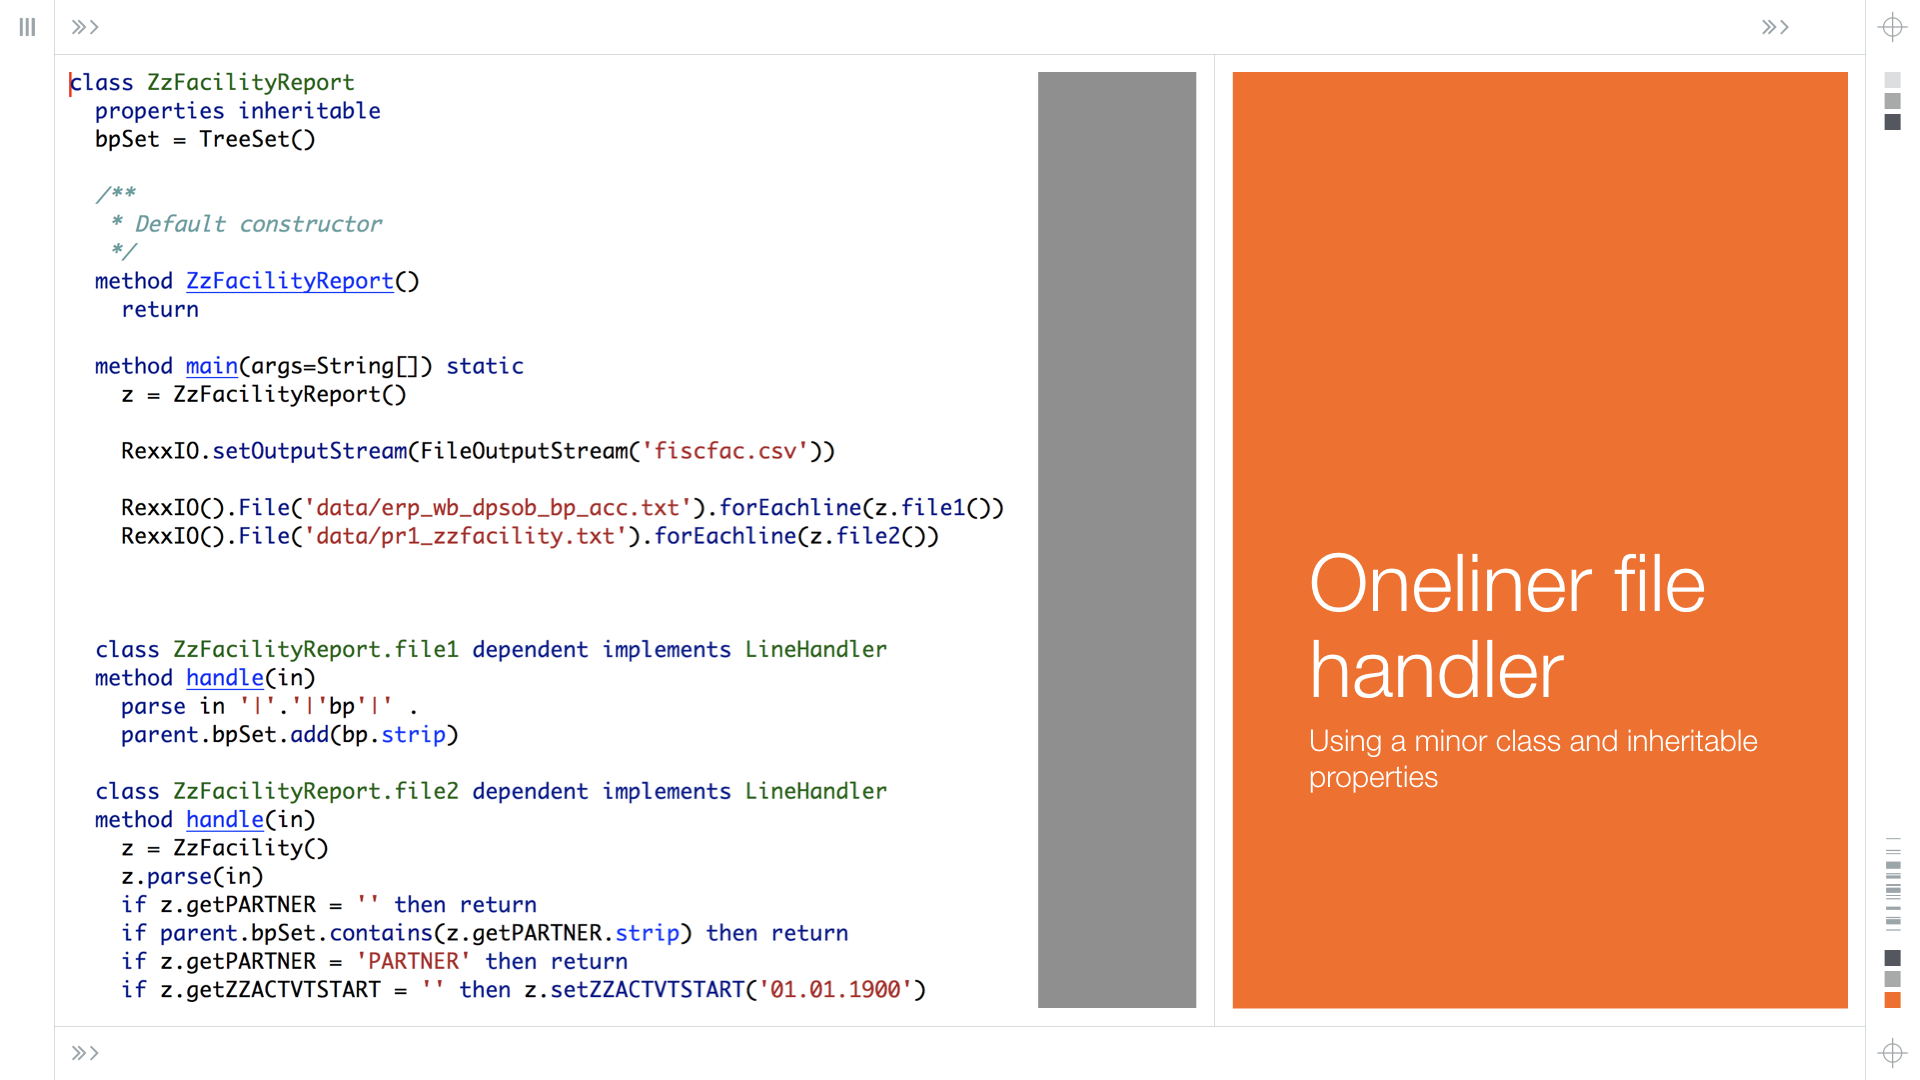
\includegraphics{NetRexx3.07.008.png}}
    \end{center}
    \caption{Oneliner file handler} \label{fig:3.07.1}
  \end{figure*}

\begin{figure*}[h]
    \begin{center}
      \scalebox{0.2}{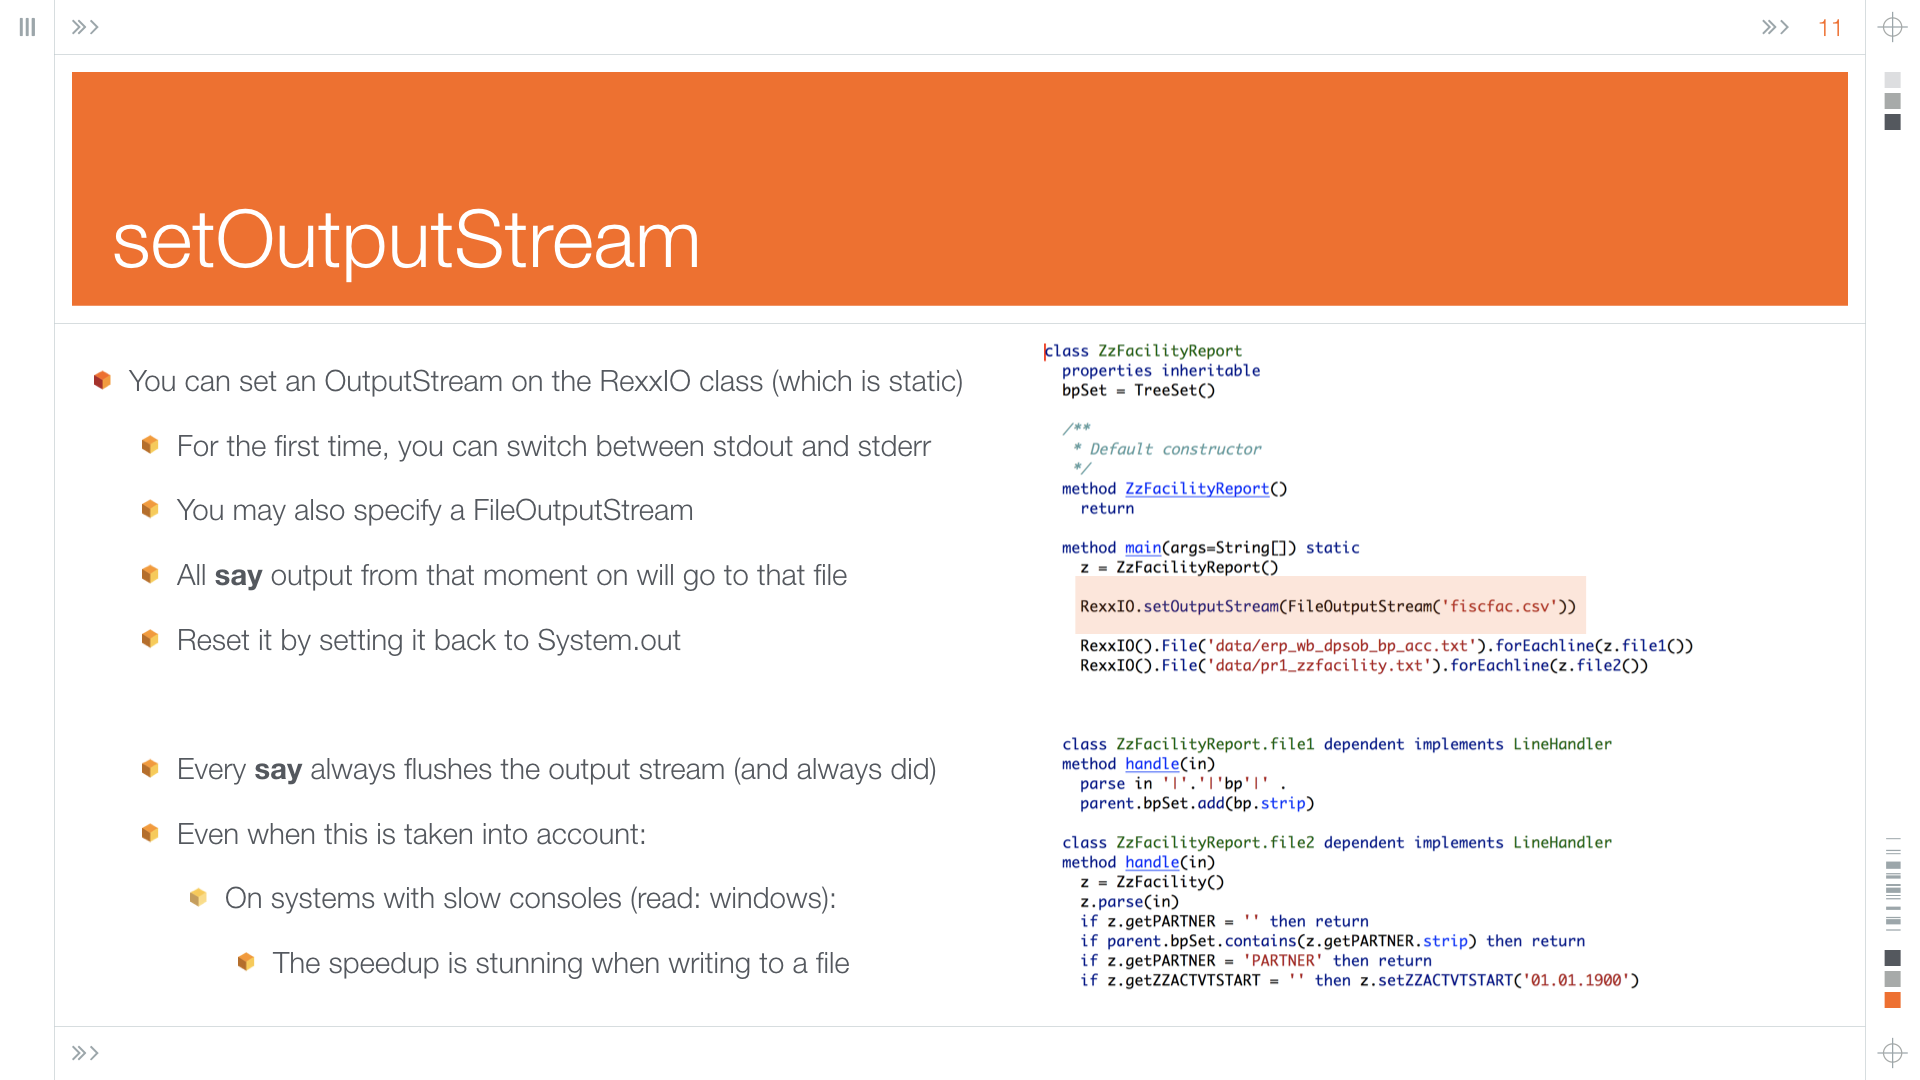
\includegraphics{NetRexx3.07.011.png}}
    \end{center}
    \caption{Set the output stream for Say} \label{fig:3.07.2}
  \end{figure*}

\begin{figure*}[h]
    \begin{center}
      \scalebox{0.2}{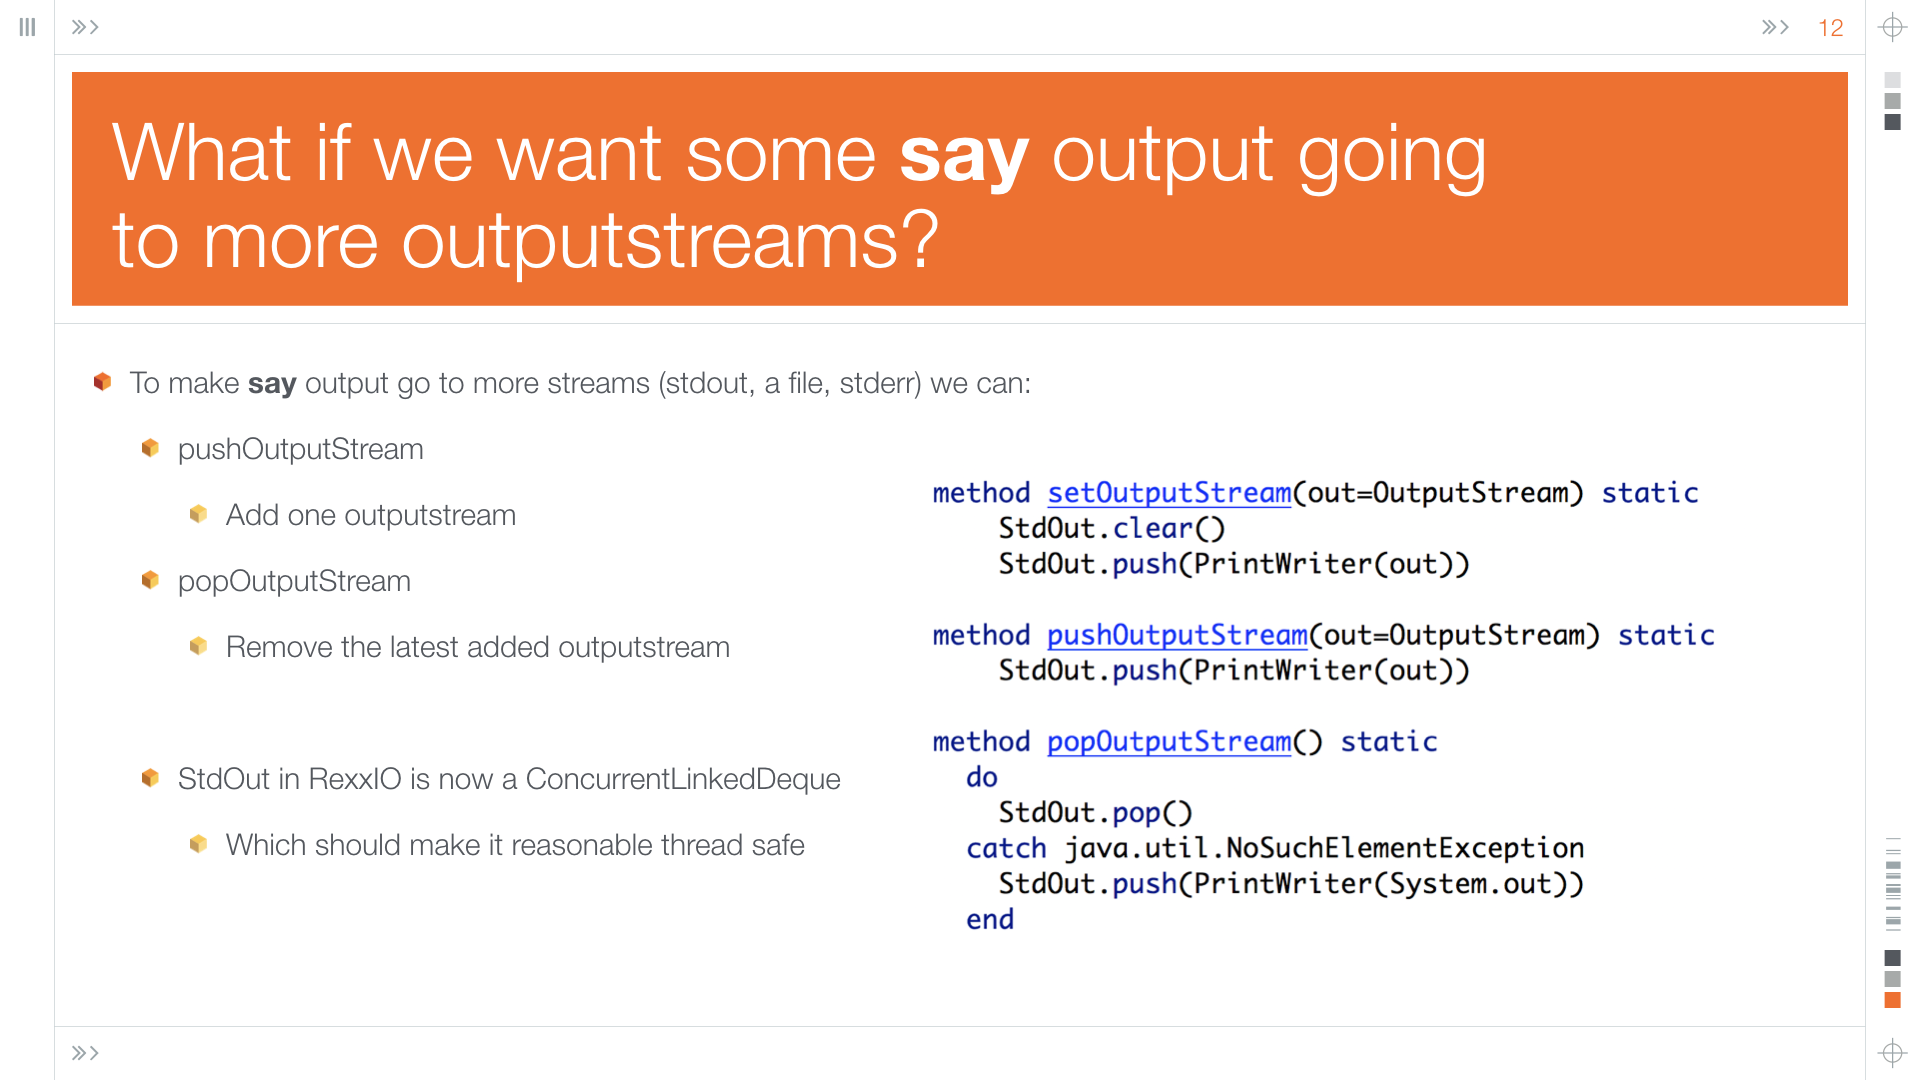
\includegraphics{NetRexx3.07.012.png}}
    \end{center}
    \caption{Using more outputstreams} \label{fig:3.07.3}
  \end{figure*}

\section{The File Class}
% \section{Streams}
% \section{Line mode I/O}
% \subsection{Line mode I/O using BufferedReader and PrintWriter}
\subsection{Line mode I/O using BufferedReader and FileOutputStream}
\lstinputlisting[label=linecomment,caption=Buffered I?O]{../../examples/ibm-historic/linecomment.nrx}
% \section{Byte Oriented I/O}
% \section{Data Oriented I/O}
% \section{Object Oriented I/O using Serialization}
% \section{The NIO Approach}
\chapter{Algorithms in \nr}{}
\section{Factorial}
A \emph{factorial} is the product of an integer and all the integers
below it; the mathematical symbol used is ! (the exclamation mark). For
example 4! is equal to 24 (because 4*3*2*1=24). The
following program illustrates a recursive (a method calling itself)
and an iterative approach to calculating factorials.
\lstinputlisting[label=factorial,caption=Factorial]{../../examples/rosettacode/RCFactorial.nrx}
Executing this program yields the following result:
\begin{verbatim}
===== Exec: RCFactorial =====
Input a number: 
42
42! = 1405006117752879898543142606244511569936384000000000 (using iteration)
42! = 1405006117752879898543142606244511569936384000000000 (using recursion)
\end{verbatim}
As you can see, fortunately, both approaches come to the same
conclusion about the results. In the above program, both
approaches are a bit intermingled; for more clarity about how to use
recursion, have a look at this:
\begin{lstlisting}[label=factorialrecursive, caption=Factorial Recursive]
class Factorial
numeric digits 64

  method main(args=String[]) static
    say factorial_(42)

  method factorial_(number) static
    if number = 0 then return 1
    else return number * factorial_(number-1)

\end{lstlisting}
In this program we can clearly see that the \texttt{factorial\_} method, that
takes an argument \texttt{number} (which is of type \Rexx{} if we do not
specify it to be another type), calls itself in the method body. This
means that at runtime, another copy of it is run, with as argument
number that the first invocation returns (the result of 42*41), and so
on.

In general, a recursive algorithm is considered more elegant, while an
iterative approach has a better runtime performance. Some language
environments are optimized for recursion, which means that their
processors can spot a recursive algorithm and optimize it by not
making many useless copies of the code. Some day in the near future
the JVM will be such an environment. Also, for some problems, for example
the processing of tree structures, using a recursive algorithm seems
much more natural, while an iterative algorithm seems complicated or forced.
\section{Fibonacci}
\lstinputlisting[label=fibonacci,caption=Fibonacci]{../../examples/rosettacode/RCFibonacciSeq.nrx}
\chapter{Using Parse}
The \texttt{Parse} statement is one of the stalwarts of the Rexx
family of languages, and allows one to easily split a string into parts without needing to resort to more traditional techniques of string processing.

The syntax of a parse statement is 

\begin{verbatim}
parse term template 
\end{verbatim}
where \texttt{term} is a string or a previously initialised variable. The template is a list of instructions describing how to split the string.

\section{Literal Parsing}
The most common use of \texttt{parse} is to split a string up into parts separated with a delimiter - whilst the most common delimiter is a simple space any string may be used:-

\begin{lstlisting}[label=SimpleParseExample, caption=Simple Parse Example]
log = "2014/05/15 21:35:47.012 - error in {{[findit]}}"
parse log year "/" month "/" day hour ":" minute ":" second "." msecond "-" text
say "On day" day "of month" month "at about" hour":"minute "we got" text
parse text "{{[" name "]}}"
say name
\end{lstlisting}

Here \texttt{log}  is composed of a datestamp separated from a message by a hyphen. The datestamp is composed of a date separated from a time by a space - within the date the year month and day are delimited by a slash and within the date the hour, minute and second fields by a colon. The millisecond field is separated from the seconds by a decimal point.

The first \texttt{parse} divides these using the relevant delimiter - where there is no delimiter then a space is used.

The \texttt{term} is the variable \texttt{log} and the \texttt{template} is 
\begin{verbatim}
year "/" month "/" day hour ":" minute ":" second "." msecond "-" text
\end{verbatim}

This first template may be read as the following sequence of actions
\begin{enumerate}
\item Assign the contents of \texttt{log} to the variable \texttt{year} until a \texttt{/} is encountered (\texttt{2014})
\item Following the \texttt{/} assign \texttt{month} with the sting found up until another \texttt{/} (\texttt{05})
\item Place the contents following the \texttt{/} until a space into the variable \texttt{day} (\texttt{15})
\item Following the space, assign the value found up until the \texttt{:} into the hour variable (\texttt{21})
\item Repeat for the variable \texttt{minute} (\texttt{35})
\item Assign the \texttt{second} value up until the \texttt{.}
\item Take the value for \texttt{msecond} until a delimiter of \texttt{-} is seen
\item Assign the remainder to variable \texttt{text}
\end{enumerate}

The second \texttt{parse} statement shows how the delimiters can be more complex - the \texttt{template} is 
\begin{verbatim}
"{{[" name "]}}"
\end{verbatim}
and extracts the value between \{\{[ and ]\}\} to the variable \texttt(name)

Running the above example will produce the following output:-
\begin{verbatim}
At about 21:35 we got  error in {{[findit]}} 
findit 
\end{verbatim}

As another example, consider
\begin{lstlisting}[label=WordSplitExample, caption=Parse Word-Split Example]
quote = "Now is the winter of our discontent"
loop forever
	parse quote word quote
	say word
	if quote = "" then leave
end
\end{lstlisting}
This will take the first word from \texttt{quote}, and assign the remainder back into \texttt{quote}, print the word taken and repeat until the variable \texttt{quote} is the empty string. The output from this will be
\begin{verbatim}
Now 
is 
the 
winter 
of 
our 
discontent
\end{verbatim}

\subsection{The Placeholder (dummy) Variable}
The first example assigns values to several variables that are not used - this is unnecessary and can be avoided by the use of a placeholder variable which is the \texttt{.} character.

If this is done, the first parse statement becomes
\begin{verbatim}
parse log . "/" month "/" day hour ":" minute ":" . "." . "-" text
\end{verbatim}
The output will remain the same.

\section{Positional Parsing}

Whilst the majority of parsing can be done using a fixed literal delimiter, the \texttt{parse} instruction also allows parsing based on positional patterns. This is achieved with the use of numerical values in the template - the values may also take a prefix of \texttt{+}, \texttt{-} or \texttt{=}

\begin{description}
\item[\texttt{no prefix} or \texttt{=}] indicates that the number is an \textbf{absolute} column value in the string being parsed
\item[\texttt{+}] indicates a \textbf{relative} position that starts from the specified position \textit{after} the position where the last match occurred
\item[\texttt{-}] indicates a \textbf{relative} position that starts from the specified position \textit{before} the last match
\end{description}

These points are best illustrated by example
\begin{lstlisting}[label=positionalParsing, caption=Positional Parsing]
quote = "Now is the winter of our discontent"
tens  = "         11111111112222222222333333"
units = "12345678901234567890123456789012345"

say quote
say tens
say units

parse quote 10 str1 20 -8 str2 +6 str3
-- str1 starts at column 10 and is 10 chars long
say  str1 "("str1.length")"
-- str2 steps back 8 chars and is 6 chars long
say str2 "("str2.length")"
-- str3 is the remainder of the string (as should be expected)
say str3
\end{lstlisting}
Running this gives the following
\begin{verbatim}
Now is the winter of our discontent 
         11111111112222222222333333 
12345678901234567890123456789012345 
e winter o (10) 
winter (6) 
 of our discontent 
\end{verbatim}

Both \texttt{literal} and \texttt{positional} parsing can be combined. Keen-eyed readers will have noted that the output from the first example contained an extra space before the word \texttt{error}
\begin{verbatim}
At about 21:35 we got  error in {{[findit]}} 
Extra space here     ^^
\end{verbatim}
This is the result of assigning the \textit{remainder} of the string to the variable text - leading blanks are normally removed \textit{except} in this special case.

One can use a positional pattern to eliminate this extra space:-
\begin{lstlisting}[label=combinedParsing, caption=Combined Parsing]
log = "2014/05/15 21:35:47.012 - error in {{[findit]}}"
parse log . "/" month "/" day hour ":" minute ":" . "." . "-" +2 text
say "On day" day "of month" month "at about" hour":"minute "we got" text
parse text "{{[" name "]}}"
say name
\end{lstlisting}

Note that the relative positional pattern used here is \texttt{+2} - \texttt{0} is the position of the last match which is the hyphen, \texttt{+1} is the position of the following space and thus \texttt{+2} is the start of the target string. 

\section{Variable Templates}
Variables may be used as the pattern in the \texttt{templates} in order to accommodate the occasions when the pattern may need to be specified at runtime. An illustration of this is the following evolution of the first example that will correctly parse dates specified in two distinct ways
\begin{lstlisting}[label=variablePattern, caption=Variables in Patterns]
log = ""
log[1] = "2014/05/15 21:35:47.012 - error in {{[findit]}}"
log[2] = "2014-05-15 21:35:47.012 - error in {{[findit]}}"

loop i = 1 to 2
	dtsep = log[i].substr(5,1)
	parse log[i] . (dtsep) month (dtsep) day hour ":" minute ":" . "." . "-" +2 text
	say "On day" day "of month" month "at about" hour":"minute "we got" text
end
\end{lstlisting}
Note that he date separator \texttt{dtsep} is determined and then used in the parse pattern by enclosing it in parentheses, thus \texttt{(dtsep)}. The output of this program is
\begin{verbatim}
On day 15 of month 05 at about 21:35 we got error in {{[findit]}} 
On day 15 of month 05 at about 21:35 we got error in {{[findit]}} 
\end{verbatim}
It can be seen that the date was successfully parsed in both cases.

It is important to note that any pattern specified by a variable \textit{will be assumed to be literal unless it has a +, - or = prefix}. Should one wish to use positional patterns then the prefix \textbf{must} be used.
\begin{lstlisting}[label=variablePosPattern, caption=Variables in Positional Patterns]
message = "this is a message that contains the number 10- just there, see?"
pat = "10"
parse message part1 5 (pat) part2
say "literal:" part1 part2
parse message part1 5 =(pat) part2
say "positional:" part1 part2
\end{lstlisting}
When run this illustrates the difference between the two parse statements
\begin{verbatim}
literal: this - just there, see? 
positional: this  message that contains the number 10- just there, see?
\end{verbatim}
\chapter{Using Trace}
The \texttt{trace} command is the inbuilt debugging facility of the \Rexx{} family, and, as might be expected from its name, allows one to trace the execution of your program. It is possible to trace both program statements and the state of variables within your code.

\texttt{(Trace)} is a compile-time option, and should be disabled once debugging as been completed.

The syntax of the trace command is
\begin{verbatim}
trace traceitem 
\end{verbatim}
where \texttt{traceitem} defines the behaviour of the trace command. Only one \texttt{traceitem} may be given, and only one of the program statement tracing options will be in use at any time. 
Variable tracing options, however, are \textit{additive} and such statements may appear multiple times.

All \texttt{trace} output is headed by three hyphens followed by the source file name, as follows
\begin{verbatim}
--- TerribleExample.nrx
\end{verbatim}

\section{Tracing Program Statements}
The \texttt{traceoptions} that affect the tracing of program statements are
\begin{description}
\item[\textbf{all}] will display all statements as they are executed. Each line in the trace output will be prefixed with \texttt{*=*} or a \texttt{*-*} should output span subsequent lines.

The \texttt{trace all} statement can be placed anywhere in the program source. 

\item[\textbf{methods}] will show the each method as it is invoked, along with any parameters to it. The trace output for method traces is prefixed by a \texttt{*=*} for the method call itself and a \texttt{>a>} indicating the assignment of a value to a method parameter. \textit{No other program statements will be traced.}

The \texttt{trace methods} statement should be placed \textit{before} the first method is defined in a class.

\item[\textbf{results}] acts as though the \texttt{trace all} statement had been given, and, if placed \textit{before} any method will also act as though \texttt{trace methods} was also specified.

In addition to the \texttt{all} and \texttt{methods} tracing implied by \texttt{results} the following will also take place
\begin{description}

\item[Properties] will have their assignments shown. These will be identified by \texttt{>p>}

\item[Local variables] will also be traced, with assignments identified by \texttt{>v>}

\item[Expressions] will have their evaluations shown if not shown for as a part of \texttt{properties} or \texttt{local variable} trace output. Such evaluations are indicated by \texttt{>>>}
\end{description}
\item[\textbf{off}] \texttt{trace off} disables tracing. No further tracing output will take place.
\end{description} 

\section{Tracing Variables}
The all-or-nothing tracing offered by, for instance \texttt{trace results} can lead to a deluge of trace information in many cases.

In these instances one may more finely control which variables one wishes to monitor using the \texttt{trace var} statement.
The syntax of the \texttt{trace var} statement is 
\begin{verbatim}
trace var var1 [var2...]
\end{verbatim}
or
\begin{verbatim}
trace var -var1 [-var2...]
\end{verbatim}
where the first form adds variables to the list that should be watched, and the second removes them. The forms may be mixed to add some variables and remove others simultaneously, as here:-
\begin{verbatim}
trace var var1 -var2 var3 -var4 -var5
\end{verbatim}
to  monitor \texttt{var1} and \texttt{var3} and remove \texttt{var2, var5} and \texttt{var5} from the list of watched variables. 

Multiple \texttt{trace var} statements may be used, as mentioned above.

It is not an error to specify a variable name that does not exist.

Each variable can appear only \textit{once} in a \texttt{trace} statement.

A variable name may that of any type - including arrays (without the \texttt{[]}).

Program tracing options never alter the list of watched variables. If tracing has previously been turned off then variable tracing may be resumed simply with a \texttt{trace var} statement.

\section{Examples}
\subsection{Program Trace}
\subsubsection{Trace All}
Running the program below
\begin{lstlisting}[label=Trace1, caption=Trace Example 1]
trace all

class traceExample   

	properties
		aIs
		bIs
	
	method traceExample(a, b)
		aIs = a
		bIs = b
		
	method times
		retturn aIs * bIs

	method main($cmdin1=String[]) static
		arg=Rexx($cmdin1)
		te = traceExample(2, 3)
		fred = te.times
		say fred
\end{lstlisting}
gives trace output of
\begin{verbatim}
     --- traceExample.nrx 
  16 *=*  method main($cmdin1=String[]) static
     >a> $cmdin1 "[Ljava.lang.String;@72ebbf5c" 
  17 *=*   arg=Rexx($cmdin1)
  18 *=*   te = traceExample(2, 3)
   9 *=*  method traceExample(a, b)
     >a> a "2" 
     >a> b "3" 
  10 *=*   aIs = a
  11 *=*   bIs = b
  12 *-* 
  19 *=*   fred = te.times
  13 *=*  method times
  14 *=*   return aIs * bIs
  20 *=*   say fred
\end{verbatim}
This output may be read thus
\begin{description}
\item[\hphantom{111}--- traceExample.nrx] Identification of the program being traced. This is the \texttt{tracing context}.
\item[16 *=*  method main(\$cmdin1=String[]) static] The first line that is actually executed is line 16.
\item[\hphantom{111}>a> \$cmdin1 "[Ljava.lang.String;@72ebbf5c"] Variable \texttt{\$cmdin1} is assigned a string value from the java virtual machine.
\item[17 *=*   arg=Rexx(\$cmdin1)]Line 17 is executed next...
\item[18 *=*   te = traceExample(2, 3)] followed by line 18
\item[\hphantom{1}9 *=*  method traceExample(a, b)] Line 18 is a method call to a method on line 9...
\item[\hphantom{111}>a> a "2"] which assigns a value of 2 to parameter a
\item[\hphantom{111}>a> b "3"] and a value of 3 to parameter b
\item[10 *=*   aIs = a] the following lines document only code execution
\item[11 *=*   bIs = b] 
\item[12 *-*] 
\item[19 *=*   fred = te.times]
\item[13 *=*  method times]
\item[14 *=*   return aIs * bIs]
\item[20 *=*   say fred]
\end{description}

\subsubsection{Trace Methods}
Replacing the \texttt{trace all} from line 1 with \texttt{trace methods} gives trace output of
\begin{verbatim}
    --- traceExample.nrx 
 16 *=*  method main($cmdin1=String[]) static
    >a> $cmdin1 "[Ljava.lang.String;@8094cc7" 
  9 *=*  method traceExample(a, b)
    >a> a "2" 
    >a> b "3" 
 13 *=*  method times
\end{verbatim}
As should be expected, this is a subset of the output provided when using \texttt{trace all}.
\subsubsection{Trace Results}
Replacing the \texttt{trace all} from line 1 with \texttt{trace results} would give
\begin{verbatim}
    --- traceExample.nrx 
 16 *=*  method main($cmdin1=String[]) static
    >a> $cmdin1 "[Ljava.lang.String;@72ebbf5c" 
 17 *=*   arg=Rexx($cmdin1)
    >>> "[Ljava.lang.String;@72ebbf5c" 
    >v> arg "" 
 18 *=*   te = traceExample(2, 3)
    >>> "2" 
    >>> "3" 
  9 *=*  method traceExample(a, b)
    >a> a "2" 
    >a> b "3" 
 10 *=*   aIs = a
    >p> aIs "2" 
 11 *=*   bIs = b
 12 *-* 
 11 >p> bIs "3"
 18 >v> te "traceExample@53606bf5"
 19 *=*   fred = te.times
 13 *=*  method times
 14 *=*   return aIs * bIs
    >>> "6" 
 19 >v> fred "6"
 20 *=*   say fred
    >>> "6" 
\end{verbatim}
Here is can be seen that more information is available. Noticeably, the values of assignments are given.
For instance
\begin{description}
\item Line 17 now has an entry of \textbf{>v> arg ""} showing that hte value of the variable \texttt{arg} was set to the empty string
\item Line 18 now has the values of the specified parameters evaluated (\mbox{\textbf{\textgreater\textgreater> "2"}} and \mbox{\textbf{\textgreater\textgreater>> "3"}})
\item Lines 10 and 11 show that values were assigned to parameters (\mbox{\textbf{>p> aIs "2"}} and \mbox{\textbf{>p> bIs "3"})}
\item Line 18 then shows the assignment of the instantiated class to variable \texttt{te}
\item Line 14 shows the evaluation of the multiplication (\mbox{\textbf{\textgreater\textgreater> "6"}}), which is assigned to variable \texttt{fred} in line 19 (\mbox{\textbf{>v> fred "6"}}) on line 19.
\item Finally we see the evaluation of variable \texttt{fred} on line 20.
\end{description}
\subsection{Variable Tracing}
Consider the following example:-
\begin{lstlisting}[label=Trace2, caption=Trace Example 2]
a = "a"
b = "b"
c = 1
d = 2
e = 3

trace var a b c d e f y
z = a || b
y = c + d
f = y + 2
e = f

trace var -a -c -d -e 
y = y * 2
a = y
e = a
\end{lstlisting}
Running this will produce the output below
\begin{verbatim}
    --- variableTraceExample.nrx 
  9 *=* y = c + d
    >v> y "3" 
 10 *=* f = y + 2
    >v> f "5" 
 11 *=* e = f
    >v> e "5" 
 14 *=* y = y * 2
    >v> y "6" 
\end{verbatim}
It can be seen that only the lines that contain watched variables are traced. This the variable assignments on lines 9, 10 and 11 are displayed, since the variables being watched from line 7 to line 12 are \texttt{a, b, c, d, e, f} and \texttt{y}.

Following this, however only the assignment to variable \texttt{y} is shown, since the variables \texttt{a, b ,c d} and \texttt{e} are removed from the list with the command \mbox{\texttt{trace var -a -c -d -e}}.

\section{Tracing Notes}
One further prefix may be encountered in the trace outout \texttt{+++} which signifies an error.

Whenever tracing transfers to a different source file, a new \texttt{tracing context}, identified by the \texttt{---} prefix is output.

Tracing is expensive, and may dramatically impact the run-time performance of the program being traced. Judicious use may therefore be warranted.

\chapter{Concurrency}
\section{Threads}
Threads are a built-in multitasking feature of the JVM. Where earlier
JVM implementations sometime ran on so-called \emph{Green Threads},
which is a library that implements thread support for OS'ses that do
not have this facility (an
early version of Java was called \emph{GreenTalk} for this reason), modern versions
all use native OS thread support. 

A new thread is created when we create an instance of the Thread class. We cannot tell a thread which method to run, because threads are not references to methods. Instead we use the Runnable interface to create an object that contains the run method:

Every thread begins its concurrent life by executing the run method. The run method does not have any parameters, does not return a value, and is not allowed to signal any exceptions.
Any class that implements the Runnable interface can serve as a target of a new thread. An object of a class that implements the Runnable interface is used as a parameter for the thread constructor.

Threads can be given a name that is visible when listing the threads in your system. It is good practice to name every thread, because if something goes wrong you can see which threads are still running.
Additionally, threads are grouped by thread groups. If you do not
supply a thread group, the new thread is added to the thread group of
the currently executing thread. The threads of a group and their
subgroups can be destroyed, stopped, resumed, or suspended by using
the ThreadGroup object. 

The next two samples are used in the following programs that
illustrate thread usage.
\lstinputlisting[label=threads1,caption=Thread sample 1]{../../examples/NrxRedBk/thread/ThrdTst1.nrx} 
\lstinputlisting[label=threads2,caption=Thread sample
2]{../../examples/NrxRedBk/thread/ThrdTst2.nrx} 
The second class, Hello2, does not \emph{implement} the
\texttt{Runnable} interface, but subclasses it, so it inherits its
methods. This is a valid approach, and it is up to the developer to
choose an implementation and worry about the semantics of an inherited
thread interface.
A newly created thread remains idle until the start method is invoked. The thread then wakes up and executes the run method of its target object. The start method can be called only once. The thread continues running until the run method completes or the stop method of the thread is called.


.* ------------------------------------------------------------------
.* NetRexx User's Guide                                              mfc
.* Copyright (c) IBM Corporation 1996, 2000.  All Rights Reserved.
.* ------------------------------------------------------------------
:h2 id=useapplet.Using NetRexx for Web applets
.pi /Web applets, writing
.pi /applets for the Web, writing
:p.
Web applets can be written one of two styles:
:ul.
:li.
.pi /binary arithmetic, used for Web applets
:q.Lean and mean:eq., where binary arithmetic is used, and only core
Java classes (such as :m.java.lang.String:em.) are used.  This is
recommended for World Wide Web pages, which may be accessed by people
using a slow dial-up connection.
Several examples using this style are included in the NetRexx package
.pi /NervousTexxt example
.pi /ArchText example
(&eg., :m.NervousTexxt.nrx:em. or :m.ArchText.nrx:em.).
:li.
:q.Full-function:eq., where decimal arithmetic is used, and advantage is
taken of the full power of the NetRexx runtime (Rexx) class.
This is appropriate for intranets, where most users will have fast
connections to servers.
An example using this style is included in the NetRexx package
.pi /WordClock example
(:m.WordClock.nrx:em.).
:eul.
:p.
If you write applets which use the NetRexx runtime (or any other Java
classes that might not be on the client browser), the rest of this
section may help in setting up your Web server.
:p.
.pi /HTTP server setup
.pi /Web server setup
.pi /runtime/web server setup
A good way of setting up an HTTP (Web) server for this is to keep all
your applets in one subdirectory.  You can then make the NetRexx runtime
classes (that is, the classes in the package known to the Java Virtual
Machine as :m.netrexx.lang:em.) available to all the applets by
unzipping NetRexxR.jar into a subdirectory :m.netrexx/lang:em. below
your applets directory.
:p.
For example, if the root of your server data tree is
:xmp.
D:/mydata
:exmp.
:pc.then you might put your applets into
:xmp.
D:/mydata/applets
:exmp.
:pc.and then the NetRexx classes (unzipped from NetRexxR.jar) should be in
the directory
:xmp.
D:/mydata/applets/netrexx/lang
:exmp.
:p.
The same principle is applied if you have any other non-core Java
packages that you want to make available to your applets: the classes in
a package called :m.iris.sort.quicksorts:em. would go in a subdirectory
below :m.applets:em. called :m.iris/sort/quicksorts:em., for example.
:p.
Note that with Java 1.1 or later it should be possible to use the
classes direct from the NetRexxR.jar file providing that the browser
being used is at a Java 1.1 level.  This may also depend on your server
being set up correctly.  Please see the Java documentation for details.
.*

\chapter{Network Programming}
\section{Using Uniform Resource Locators (URL)}
\section{TCP/IP Socket I/O}
\section{RMI: Remote Method Interface}

\chapter{Database Connectivity with JDBC}
For interfacing with Relational Database Management Systems (RDBMS)
\nr{} uses the Java Data Base Connectivity (JDBC) model. This means
that all important database systems, for which a JDBC driver has
been made available, can be used from your \nr{} program. This is a
large bonus when we compare this to the other open source scripting
languages, that have been made go by with specific, nonstandard
solutions and special drivers. In contrast, \nr{} programs can be
made compatible with most database systems that use standard SQL, and,
with some planning and care, can switch database implementations at
will.
\lstinputlisting[label=jdbc,caption=A JDBC Query example]{../../examples/NrxRedBk/jdbc/JdbcQry.nrx} 

The first peculiarity of JDBC is the way the driver class is
loaded. When most classes are 'pulled in' by the translator, a JDBC
driver traditionally is loaded through the reflection API. This
happens in line 22 with the \texttt{Class.forName} call. This implies
that the library containing this class must be on the classpath.

\begin{shaded}\noindent
In previous versions of JDBC, to obtain a connection, one first had to
initialize the JDBC driver by calling the method Class.forName. Any
JDBC 4.0 drivers that are found on the class path are automatically
loaded. (However, one must manually load any drivers prior to JDBC 4.0
with the method Class.forName.)
\end{shaded}\indent

In line 32 of the example we connect to the database using a url and a
userid/password combination. This is an easy way to do and test, but
for most serious applications we do not want plaintext userids and
passwords in the sourcecode, so most of the time we would store the
connection info in a file that we store in encrypted form, or we use
facilities of J2EE containers that can provide data sources that take
care of this, while at the same time decoupling your application
source from the infrastructure that it will run on.

In line 47 the query is composed by filling in variables in a Rexx
string and making a \texttt{Statement} out of it, in line 50. In line
  55, the \texttt{Statement} is executed, which yields a
  \texttt{ResultSet}. This has a \emph{cursor} that moves forward with
  each \texttt{next} call. The \texttt{next} call returns \emph{true}
  as longs as there are rows from the resultset to return.

The \texttt{ResultSet} interface implements \emph{getter} methods for
  all JDBC Types. In the above example, all returned results are of
  type \texttt{String}.

\lstinputlisting[label=jdbcu,caption=A JDBC Update
example]{../../examples/NrxRedBk/jdbc/JdbcUpd.nrx} 
For database updates, we connect using the driver in the same way
(line 23) and now prepare the statement used for the database update
(line 50). In this example, we loop through the cursor of a select
statement and update the row in line 66. The \texttt{executeUpdate}
method of \texttt{PreparedStatement} returns the number of updated
rows as an indication of success.

From JDBC 2.0 on, cursors are updateable (and scrollable, so they can
move back and forth), so we would not have to go
through this effort - but it is a valid example of an update statement.
\chapter{WebSphere MQ}
WebSphere MQ (also and maybe better known as MQ Series) is IBM's
messaging and queing middleware, and is in use at a great many financial
institutions and other companies. It has, from a programming point of
view, two API's: JMS (Java Messaging Services), a generic messaging
API for the Java world, and MQI, which is older and proprietary to
IBM's product. The below examples show the MQI; other examples might
show JMS applications.

This is the sample Java application for MQI, translated (and a lot
shorter) to NetRexx.
\lstinputlisting[label=mqsample,caption=MQ Sample]{../../examples/enterprise/wmq/MQSample.nrx}
This sample connects to the Queue Manager (called \emph{rjtestqm}) in
\emph{bindings mode}, as opposed to \emph{client mode}. Bindings mode
is only a connection possibility for client programs that are running
in the same OS image as the Queue Manager, on the server. Note that
the application connects (line 19), accesses a queue (line 23), puts a
message (line 32), gets it back (line 39) closes the queue (line 45) and disconnects (line 48) all without checking
returncodes: the exceptionhandler takes care of this, and all
irregulaties will be reported from the catch MQException block
starting at line 50).

The main method does in this case not follow the canonical form, but
has 'binary' as an extra option. Option binary can be defined on the
command line as an option to the translator, as a program option, as a
class option and as a method option. Here the smallest scope is
chosen. There is a good reason to make this method a binary method:
accessing a queue in MQ Series requires some options that are set
using a mask of binary flags - this works, in current \nr{} versions,
only in binary mode, because the operators have other semantics in
nobinary mode.

\lstinputlisting[label=mqlistener,caption=MQ Message Reader]{../../examples/enterprise/wmq/MessageReader.nrx}
In contrast to the previous sample the MessageReader sample only has
one import statement. This is always hotly debated in project teams,
one school likes the succinctness of including only the top level
import, and only goes deeper when there is ambiguity detected; another
school spells out the all imports to the bitter end. 

The MessageReader sample connects to another queue, called TESTQUEUE1
(specified in line 7) but here we connect in \emph{client mode}, as
indicated by lines 13-15 which specify an MQEnvironment. Other
options are using an MQSERVER environment variable or a \emph{Channel
Definition Table}.

This program is also uncommon in that it uses
\texttt{MQConstants.MQGMO\_WAIT} as an option instead of being
triggered as a process by a message on a trigger queue. Using this
option means that the program waits (stays active, not really busy polling
but depending on an OS event) until a new
message arrives, which will be processed immediately.

In lines 18-21 a \emph{Channel Exit} is specified. This exit is show
in the following example.
\lstinputlisting[label=mqjavachannelexit,caption=MQ Java Channel Exit]{../../examples/enterprise/wmq/TimeoutChannelExit.nrx}
 \lstinputlisting[label=watchdogtimer,caption=WatchdogTimer]{../../examples/enterprise/wmq/WatchdogTimer.nrx}
MQ Series has traditional channel exits (programs that can look at the
message contents before the application gets to it). In the MQI Java
environment there is something akin to this functionality, but a Java
channel exit for MQ Series has to be defined in the application, as
shown in the previous example. The function of this particular exit is
to implement a \emph{Watchdog timer} - on a separate thread, as shown
in the sample that follows the sample channel exit. The timer
threatens here to have issues a HP OpenView alert, but that part has
been left out.

This particular sample has been designed to do something that is
normally a bit harder
to do: signal the operations department when something does NOT happen
- here the assumption is that there is a payment going over the queue
at least once every 20 minutes - when that does not happen, an alert
is issued. With every message that goes through, the timer thread is
reset, and only when it is allowed to time out, action is undertaken.

\lstinputlisting[label=watchdogtimer,caption=Publish/Subscribe]{../../examples/enterprise/wmq/MQPubSubSample.nrx}
This sample shows the publish-subscribe interfaces that at some time have been
added to the product. This specific sample shows some Java thread
complexity but is a good example of doing publish/subscribe work in a
multithreaded way, which is a natural fit for this type of work.

\chapter{MQTT}\label{mqtt}
 
 
\section{Pub/Sub with MQ Telemetry }
 
Publish/subscribe (pub/sub) is a model that lends itself very well to a number of one publisher, many subscriber type of applications; the tools to enter this technology have never been as available as they are now. Also, MQTT is a small protocol that needs to be taken seriously: Facebook has recently become one of the largest users.
 
Designed as a low-overhead on-the-wire protocol for brokers in the Internet-of-things age, MQTT is an exciting new development in the Messaging and Queueing realm. It is a good choice for any broker functionality, as the minimal message overhead is 2 bytes, but the maximum messages size, in one of the more popular open source brokers is a good 250MB, which give you a message size that is a lot higher than anything possible in the early years of MQ Series back in the nineties. It is now possible to do development with an entry level, entirely open source suite, and scale up to commercial, clustered and highly available implementations when needed, since the protocol has is supported by the base IBM WebSphere MQ product and is an added deliverable in WSMQ 7.5, after being available as an installable add-on for several years.
 
Here I will show how extremely straightforward it is to create a pub/sub application using this technology. These examples use NetRexx, the Eclipse PAHO Java client library and the open source Mosquitto broker; all these components are completely free and open source. I have installed Mosquitto on my MacBook using the brew system(fn), which makes it as much trouble as “sudo brew install mosquitto”.  NetRexx is an excellent language for these examples, as it is compact and avoids the C-inspired ceremony of Java language syntax; if your project requires Java, you can just save the generated Java source (using the new –keepasjava option).
 
Mosquitto(fn) is written by Roger Light as an open source equivalent of IBM’s rsmb (real small message broker) example application, which is free but lacks source code. It is a small broker application that nevertheless runs production sized workloads. As MQTT, as opposed to the MQI or JMS API’s you use when developing a messaging application, is an on-the-wire protocol (commercial messaging systems tend to have their own, unpublished, on-the-wire protocols), we need an API to use it. This API consists of a set of calls that do the formatting of the messages to the requirements of the on-the-wire protocol for you. The messages themselves are just byte-arrays, which gives you the ultimate freedom in designing their content. It is not unusual for connected devices to encode their information in a few bits; on the other hand, there is no reason not to use extreme verbosity in messages; as long as you send the .getBytes that your String yields, MQTT will send it. When encoding information in a compact way, the protocol design will really pay off, because the protocol overhead, in comparison with http and other chatty protocols, is very low. A limited set of quality of service options (qos) will indicate if you want send and pray, acknowledged delivery or acknowledged one-time-only delivery.
 
The API library that was chosen for these examples is that from the Eclipse PAHO project. This project, which is in its early stages, has C, Javascript and Java client libraries available. I chose the Java client because the JVM environment is where most of the organizations that I work for will use it. The PAHO Java client library is donated by IBM and written by Dave Locke; it is in active development. If you want to see how the protocol moves in packets over the network, I can recommend Wireshark, which does a good job of recognizing them (if you run on the standard port 1883) and showing you the message types (like ACK) and their bytes.
 
After having put the NetRexx(.jar) and paho client jars on your classpath, you are good to go. The first example here is the publisher – this is not a fragment, but the complete code. For production code we might add some more checks, as enterprise environments always are prone to suddenly run low on disk space and suffer missing authorizations, but it works as it stands. Do note that you do not have to define a message topic in advance – just think of one any use it, at least if you are in your own environment. With Mosquitto, there wasn’t anything to define in advance, and the running Publisher (happily lifted from the Java example) in NetRexx was actually the first time I talked to Mosquitto on my MacBook.
 
\lstinputlisting[label=mqlistener,caption=MQTT Publish Sample]{../../../../examples/enterprise/mqtt/Publish.nrx}
 
Topics can have a hierarchical organization; this structure is put in by composing trees of topics, which are strings separated by ‘/’. In this way, it is easy to compose a /news/economics/today topic string that gives some structure to the publication. The classification is entirely up to the designer.
 
Messaging in its original form is an asynchronous technology, and for this reason the API offers a callback option, where the callback receives the results of your publish action in an asynchronous way. The broker assigns a message id which you receive back.
 
 
The second source fragment (and again, it is no fragment but the entire application program) shows the subscriber.
 
\lstinputlisting[label=mqlistener,caption=MQTT Subscribe Sample]{../../../../examples/enterprise/mqtt/Subscribe.nrx}
  
Security is outside of the scope of this introduction which shows you the sourcecode of a simple pub/sub application, but in Mosquitto the traffic can be secured using SSL certificates and userid/password combinations; also, the access to topics can be limited. In terms of availability, the Mosquitto configuration file offers an opportunity to send all messages for a defined set of topics to another connected broker, which might be in a different part of the world, or your home, to enable a redundant setup. While the broker does not offer the queue – transmission queue - channel setup with retrying channels that MQ does, the client API has some facilities to locally save the messages and retry if the communication was lost. Also, the last-will-and-testament facility is something that traditional MQ does not have.
 
 


\chapter{Component Based Programming: Beans}
JavaBeans is the name for the Java component model. It consists of two
conventions, for the naming of \emph{getter} and \emph{setter} methods
for properties, and the \emph{event} mechanism for sending and
receiving events. \nr{} adds support for the automatic generation of
getter and setter methods, throught the \textbf{properties indirect}
option on the properties statement.
% .* ------------------------------------------------------------------
% .* \nr{} User's Guide                                              mfc
% .* Copyright (c) IBM Corporation 1996, 2000.  All Rights Reserved.
% .* ------------------------------------------------------------------
\chapter{Using the \nr{}A API}\label{api}
\index{interpreting,API}
\index{interpreting,using the \nr{}A API}
\index{application programming interface, for interpreting}
\index{\nr{}A, class}
\index{\nr{}A, API}
\index{ref /API/application programming interface}
As described elsewhere, the simplest way to use the \nr{} interpreter
is to use the command interface (\nr{}C) with the \emph{-exec}
or \emph{-arg} flags.
There is a also a more direct way to use the interpreter when calling it
from another \nr{} (or Java) program, as described here.  This
way is called the \emph{\nr{}A Application Programming Interface}
(API).
\newline
The \emph{\nr{}A} class is in the same package as the translator
(that is, \emph{org.netrexx.process}), and comprises a constructor
and two methods.  To interpret a \nr{} program (or, in general, call
arbitrary methods on interpreted classes), the following steps are
necessary:
\begin{enumerate}
\item Construct the interpreter object by invoking the constructor \emph{\nr{}A()}.
At this point, the environment's classpath is inspected and known
compiled packages and extensions are identified.
\item Decide on the program(s) which are to be interpreted, and invoke the
\nr{}A \emph{parse} method to parse the programs.  This parsing
carries out syntax and other static checks on the programs specified,
and prepares them for interpretation.  A stub class is created
and loaded for each class parsed, which allows access to the classes
through the JVM reflection mechanisms.
\item At this point, the classes in the programs are ready for use.  To invoke
a method on one, or construct an instance of a class, or array, etc.,
the Java reflection API (in \emph{java.lang} and \emph{java.lang.reflect})
is used in the usual way, working on the \emph{Class} objects created by
the interpreter.  To locate these \emph{Class} objects, the
API's \emph{getClassObject} method must be used.
\end{enumerate}

Once step 2 has been completed, any combination or repetition of using
the classes is allowed.  At any time (provided that all methods invoked
in step 3 have returned) a new or edited set of source files can be
parsed as described in step 2, and after that, the new set of class
objects can be located and used.  Note that operation is undefined if
any attempt is made to use a class object that was located before the
most recent call to the \emph{parse} method.
\newline
Here's a simple example, a program that invokes the \emph{main} method
of the \emph{hello.nrx} program's class:
\index{interpreting/API example}
\begin{lstlisting}[label=netrexxa,caption=Try the \nr{}A interface]
options binary
import org.netrexx.process.\nr{}A

interpreter=NetRexxA()             -- make interpreter

files=['hello.nrx']                -- a file to interpret
flags=['nocrossref', 'verbose0']   -- flags, for example
interpreter.parse(files, flags)    -- parse the file(s), using the flags

helloClass=interpreter.getClassObject(null, 'hello') -- find the hello Class

-- find the 'main' method; it takes an array of Strings as its argument
classes=[interpreter.getClassObject('java.lang', 'String', 1)]
mainMethod=helloClass.getMethod('main', classes)

-- now invoke it, with a null instance (it is static) and an empty String array
values=[Object String[0]]

loop for 10    -- let's call it ten times, for fun...
  mainMethod.invoke(null, values)
end
\end{lstlisting}

Compiling and running (or interpreting!) this example program will
illustrate some important points, especially if a \textbf{trace all}
instruction is added near the top.  First, the performance of the
interpreter (or indeed the compiler) is dominated by JVM and other
start-up costs; constructing the interpreter is expensive as the
classpath has to be searched for duplicate classes, etc.  Similarly,
the first call to the parse method is slow because of the time taken to
load, verify, and JIT-compile the classes that comprise the interpreter.
After that point, however, only newly-referenced classes require
loading, and execution will be very much faster.
\newline
The remainder of this section describes the constructor and the two
methods of the \nr{}A class in more detail.
%.*
%.* - - - - -
%.cp 8
\section{The NetRexxA constructor}
\index{NetRexxA/constructor}
\index{constructor, in NetRexxA API}

\begin{lstlisting}[label=constructor,caption=Constructor]
NetRexxA()
\end{lstlisting}
This constructor takes no arguments and builds an interpeter object.
This process includes checking the classpath and other libraries known
to the JVM and identifying classes and packages which are available.
%.* - - - - -
%.cp 8
\section{The parse method}
\index{parse method, in \nr{}A API}
\begin{lstlisting}[label=parse,caption=parse]
parse(files=String[], flags=String[]) returns boolean
\end{lstlisting}

The parse method takes two arrays of Strings.  The first array contains
a list of one or more file specifications, one in each element of the
array; these specify the files that are to be parsed and made ready for
interpretation.
\newline
The second array is a list of zero or more option words; these may be
any option words understood by the interpreter (but excluding those
known only to the \nr{}C command interface, such as \emph{time}).
\footnote{Note that the option words are not prefixed with a \emph{-}.}
The parse method prefixes the \emph{nojava} flag automatically, to
prevent \emph{.java} files being created inadvertently.  In the
example, \emph{nocrossref} is supplied to stop a cross-reference file
being written, and \emph{verbose0} is added to prevent the logo and
other progress displays appearing.
\newline
The \emph{parse} method returns a boolean value; this will be 1 (true)
if the parsing completed without errors, or 0 (false) otherwise.
Normally a program using the API should test this result an take
appropriate action; it will not be possible to interpret a program or
class whose parsing failed with an error.

\section{The getClassObject method}
\index{getClassObject method, in \nr{}A API}

\begin{lstlisting}[label=getclassobject,caption=getClassObject]
getClassObject(package=String, name=String [,dimension=int]) returns Class
\end{lstlisting}

This method lets you obtain a Class object (an object of
type \emph{java.lang.Class})  representing a class (or array) known to
the interpreter, including those newly parsed by a parse instruction.
\newline
The first argument, \emph{package}, specifies the package name (for
example, \emph{com.ibm.math}).  For a class which is not in a
package, \emph{null} should be used (not the empty string, \emph{''}).
\newline
The second argument, \emph{name}, specifies the class name (for example,
\emph{BigDecimal}).  For a minor (inner) class, this may have
more than one part, separated by dots.
\newline
The third, optional, argument, specifies the number of dimensions of
the requested class object.  If greater than zero, the returned class
object will describe an array with the specified number of dimensions.
This argument defaults to the value 0.
\newline
An example of using the \emph{dimension} argument is shown above where
the \emph{java.lang.String[]} array Class object is requested.
\newline
Once a Class object has been retrieved from the interpreter it may be
used with the Java reflection API as usual.  The Class objects returned
are only valid until the parse method is next invoked.


\chapter{Interfacing to Scripting Languages}
\nr{} contains standardized Java Scripting
support\marginpar{\color{gray}3.03}, and the NetRexxC.jar file is a self-contained JSR223 scripting engine. This facility opens up a number of possibilities to interface in a standardized manner with several scripting languages and other infrastructure, and offers an easy way for including intrepreted \nr{} code in JVM applications. JSR223 is a standard for interacting with scripting languages that consists of:
\begin{enumerate}
\item A mechanism to find out for which scripting languages support is
  available
\item A way to choose one of them
\item An eval() call to dynamically specify and execute a program
\item A \emph{bindings} mechanism to bind variable names to values, to exchange objects with scripts
\item Optionally, a way to execute methods, functions or routines from
  larger programs
\item Optionally, a way to keep already compiled scripts around for repeated execution (with associated higher performance)
\end{enumerate}

The JSR223 specification\footnote{\url{http://www.jcp.org/en/jsr/detail?id=223}}
details the calls that are available in the \keyword{javax.scripting}
package. To use the JSR223 interface, Java 6 or higher is
required. The JAR file specification defines a service as a well-known
set of interfaces and (usually) abstract classes. A service provider
is a specific implementation of such a service. For scripting, the
service consists of \keyword{javax.script.ScriptEngineFactory}. All
classes that implement this interface are service providers. Service
providers identify themselves by placing a so-called
provider-configuration file in META-INF/services. Its filename
corresponds to the fully qualified name of the service class, which is
\keyword{javax.script.ScriptEngineFactory}. Each line of this file contains the
fully qualified name of a service provider. The factory
class of the \nr{} connector is \keyword{org.netrexx.jsr223.NetRexxScriptEngineFactory}. So the file \keyword{META-INF/services/javax.script.ScriptEngineFactory} contains one line with exactly this class name.
\section{Which JSR223 engines are on my system?}
The number of JSR223 engines available varies per JVM implementation. The following code can be used to list these.
\begin{lstlisting}[label=enumeratejsr223,caption=Enumerate the JSR223 Engines on a JVM]
import javax.script.

class ScriptDemo
  
  method main(args=String[]) static
    
    sem=ScriptEngineManager()
    list = sem.getEngineFactories()
    f=ScriptEngineFactory
    
    loop i          = 0 to list.size-1
      f             = ScriptEngineFactory list.get(i)
      engineName    = f.getEngineName()
      engineVersion = f.getEngineVersion()
      langName      = f.getLanguageName()
      langVersion   = f.getLanguageVersion()
      say engineName engineVersion langName langVersion
   end -- loop i

\end{lstlisting}
For example, the Java 8 SE version by Oracle on MacOSX delivers out of the box:
\begin{alltt}
AppleScriptEngine 1.1 AppleScript 2.2.4
Oracle Nashorn 1.8.0  ECMAScript ECMA - 262 Edition 5.1
\end{alltt}
As one can see, the name of the engine, the language and its release are standard features for this query. The NetRexxC.jar file on the classpath adds the \nr{} implementation:
\begin{alltt}
NetRexx Script Engine V1.0.0 NetRexx \nrversion{}
\end{alltt}
There can be any number of additional jar archives on the classpath to deliver engines for different JSR223 implementations for different languages.
\section{Selecting an engine}
When developing a program one is probably interested in using a specific implementation, and it is possible to request the loading of a specific JSR223 engine by name.
\begin{lstlisting}[label=choosingjsr223,caption=Choosing an engine]
import javax.script.

manager = ScriptEngineManager()
nrEngine = manager.getEngineByName("NetRexx")
\end{lstlisting}
The language engine can be selected by its short name, so there is no need to specify the longer name or its version.
\section{Evaluating a script}
This example shows how to do a simple thing that illustrates the value of being able to do this from other environments: calculating some number with \emph{numeric precision} set to some value that other languages cannot handle.
\begin{lstlisting}[label=evaljsr223,caption=Evaluating a script]
/* simple script invocation */
nrEngine.eval('numeric digits 17; say 111111111 * 111111111')
\end{lstlisting}
The output from this script would be:
\begin{alltt}
12345678987654321
\end{alltt}
\section{Bindings}
Bindings are name-value pairs whose keys are strings - they can be of \Rexx{} type. Their behavior is defined through the \keyword{javax.script.Bindings} interface. As for \keyword{ScriptContext}, a basic implementation is provided called \keyword{SimpleBindings}. Although bindings belong to script contexts, \keyword{ScriptEngine} provides \keyword{createBindings()}, which returns an uninitialized binding. Another method, \keyword{getBindings()}, exists to return the bindings of a certain scope. There are at least two scopes, \keyword{ScriptContext.GLOBAL\_SCOPE} and \keyword{ScriptContext.ENGINE\_SCOPE}. They represent key-value pairs that are either visible to all instances of a script engine that have been created by the same \keyword{ScriptengineManager}, or visible only during the lifetime of a certain script engine instance. The following program illustrates the use of bindings to store a value, 42, into the binding called \keyword{answer} and then using its retrieved value in the evaluation of the statement \keyword{'say ``the answer is'' answer '}. The next action uses the handle \keyword{one} for a value of 1, and uses its retrieved value to add it to the value previously contained in the binding \keyword{answer}.
\begin{lstlisting}[label=bindingsjsr223,caption=Object Bindings]
import javax.script.
nrEngine = ScriptEngineManager().getEngineByName("NetRexx")

/* script invocation with bindings */
answer = 42
nrEngine.put("answer", answer)
nrEngine.eval('say ''the answer is ''answer')

one = 1
nrEngine.put("onemore",one)
nrEngine.eval('say ''one more is ''answer+onemore')
\end{lstlisting}
Note that in line two, the invocation is shortened a bit by getting rid of the intermediate \keyword{manager} object for instantiation of the language interface. Also note that in line 10, we chose, for illustration purposes, to store the \keyword{one} object into the bindings structure using a different name, \keyword{onemore}. This shows that the string used as identifier for the object is just a handle to it, and nothing more.
This would yield:
\begin{alltt}
the answer is 42
one more is 43
\end{alltt}
The different possibilities and language combinations will be discussed in the paragraphs below.
 
\section{Interpreted execution of \nr{} scripts from NetRexx}
 
\section{Interpreted execution of \nr{} scripts from Java}
 
\section{Calling other scripting languages from \nr{} programs}
 
\subsection{Calling Javascript (ECMAScript, Rhino, V8, Nashorn, …) from \nr{} programs}
 
\subsection{Using AppleScript on MacOSX}
 
\section{Execution of \nr{} scripts from ANT tasks}
 
\section{Integration of NetRexx scripting in applications}
 
\section{Interfacing between ooRexx and \nr{} using BSF4ooRexx}
BSF is a system for language interaction that originated in a research project at IBM, and predates JSR223 (and certainly its implementation in Java 6) for a number of years. BSF 2.x has its own interface, while modern BSF versions are an implementation of the JSR223 interfaces. BSF4ooRexx enables a bidirectional interface between ooRexx and Java, and enables one to use the large class library support for Java in ooRexx programs, but likewise the execution of ooRexx code from Java (including \nr{}) programs. BSF4ooRexx contains some special support for JVM programs written in \nr{}.


\chapter{\nr{} Tools}
\section{Editor support}\label{editors}
This chapter lists editors that have plugin support for \nr{},
ranging from syntax coloring to full IDE support (specified), and
\Rexx{} friendly editors, that are extensible using \Rexx{} as a macro
language (which can be the first step to provide \nr{} editing support).
\subsection{JVM - All Platforms}
\begin{tabularx}{\textwidth}{>{\bfseries}lX}
\toprule
JEdit & Full support for \nr{} source code editing, to be found at
\url{http://www.jedit.org}.
\\\midrule
NetRexxDE & A revisions with additions of the \nr{} plugin for
jEdit, moving to a full IDE for \nr{}. \url{http://kenai.com/projects/netrexx-misc} 
\\\midrule
Eclipse & Eclipse has a \nr{} plugin that provides a complete IDE
environment for the development of \nr{} programs (in alpha release)
by Bill Fenlason. The project is situated at SourceForge
(\url{http://eclipsenetrexx.sourceforge.net/}). Chapter
\ref{setupeclipse} on page \pageref{setupeclipse} discusses the setup
of Eclipse to build the translator itself; and has
instructions for the setup of the \nr{} plugin.
\\\bottomrule
\end{tabularx}
\subsection{Linux}
\begin{tabularx}{\textwidth}{>{\bfseries}lX}
\toprule
Emacs & netrexx-mode.el (in the \nr{} package in the \texttt{tools}
directory) runs on GNU Emacs, which is installed by default on most
Linux developer distributions.
\\\midrule
vim & vi with extensions
\\\bottomrule
\end{tabularx}
\subsection{MS Windows}
\begin{tabularx}{\textwidth}{>{\bfseries}lX}
\toprule
Emacs & netrexx-mode.el (in the \nr{} package in the \texttt{tools} directory) runs on GNU Emacs for
Windows. \url{http://www.gnu.org/software/emacs/windows/faq.html}.
\\\midrule
vim & vi with extensions
\\\bottomrule
\end{tabularx}
\subsection{macOS}
\begin{tabularx}{\textwidth}{>{\bfseries}lX}
\toprule
Aquamacs & A version of Emacs that is integrated with the macOS Aqua
look and feel. (\url{http://www.aquamacs.org}). \nr{} mode is
included in the \nr{} package in the \texttt{tools} directory.
\\\midrule
Emacs & netrexx-mode.el (in the \nr{} package) runs on GNU Emacs for
macOS. \url{http://www.gnu.org/software/emacs}.
\\\midrule
Vim & Vi with extensions
\\\bottomrule
\end{tabularx}
\section{Java to Nrx (java2nrx)}
When working on a piece of Java code, or an example written in the
language, sometimes it would be good if we could see the source in
\nr{} to make it more readable. This is exactly what \emph{java2nrx}
by Marc Remes does. It has a  Java 1.5 parser and an Abstract Syntax
Tree that delivers a translation to NetRexx, to the
extend of what is currently supported under NetRexx.

At the moment it is to be found at \url{git clone git://git.code.sf.net/p/netrexx/code netrexx-code} in the tools directory.

It is started by the \texttt{java2nrx.sh} script; for convenience, place \texttt{java2nrx.sh} and \texttt{java2nrx.jar} in the
same directory. NetRexxC and java must be available on the path.

Usage:
\begin{rail}
java2nrx : ('java -jar java2nrx.jar' infile.java out.nrx?  
                )
               ;
\end{rail}

Alternatively:
\begin{figure}[h]
\caption{Java2nrx 2}
\begin{rail}
java2nrx : ('java2nrx.sh/.bat' 
                 ('-nrc' |'-stdout' |'-run'| options[other NetRexxC options])? filename.java 
                )
               ;
\end{rail}
\end{figure}
\begin{description}
   \item[-nrc]      runs NetRexxC compiler on output nrx file
   \item[-stdout]   prints NetRexx file on stdout
   \item[-run]      runs generated translated NetRexx output file
\end{description}

\chapter{Using Eclipse for NetRexx Development}\label{setupeclipse}
 
This is a guide for first time Eclipse users to set up a NetRexx
development project.  It is not a beginners guide to Eclipse, but is
intended to explain how to download the NetRexx compiler source from
SVN to be able to modify and build it using Eclipse\footnote{If you
  have questions or comments, feel free to contact Bill Fenlason at billfen@hvc.rr.com.}.
 
It is detailed and hopefully foolproof for someone who has never used
Eclipse.  It assumes a Windows user, but if you are a Linux or Mac
user, you will no doubt understand what to do.
 
This guide is for Eclipse 4.2 (Juno), written August, 2012.  New
Eclipse releases occur every 4 months, so there may be differences
depending on what the current version is.
 
\section{Downloading Eclipse}
 
There are many different preconfigured versions of Eclipse.  As you
become more experienced with it you may wish to use a different
distribution, but the one specified here makes some things simple.  It
does contain some things that you may never use.
\begin{enumerate}
\item Make a new folder for the project.  Name it appropriately
   (e.g. EclipseNetRexx)
\item Browse to eclipse.org, and click on ``Download''.
\item Download the version namedECLIPSE IDE FOR JAVA DEVELOPERS for your
   your operating system.
\item The download is about 150 MB.
\item Unzip the downloaded file into your project folder.
\end{enumerate}
\section{Setting up the workspace}
 
There are different strategies for managing Eclipse workspaces.
Eclipse defaults to putting the workspace in your Windows documents
folder - probably not what you want to do.  The following is perhaps
the most simple way.
\begin{enumerate}
\item Open the project folder.  It will now contain a folder named
   eclipse.
\item Add a new folder named ``workspace'' in the project folder to go
along with the eclipse folder.
\item Open the eclipse folder, and create a shortcut to eclipse.exe.
\item Move the shortcut to the desktop and rename it to something like
   ``Eclipse NetRexx''.
\item Close the project folder, and double click the shortcut to start
   Eclipse.
\item The ``Select a workspace'' dialog comes up - don't use the default.
\item Browse to the workspace folder that you just created and select it.
\item Click (check) the ``Use this as the default'' box, and click OK.
\end{enumerate}
\section{Shellshock}
 
If you have never used Eclipse, it can be a bit overwhelming.  It is
rather complicated, and has endless options, etc.  In addition there
are at least a thousand different plugins.
 
You will be greeted by a Welcome screen - you may find it interesting
or boring.  Exit from it via tback to the welcome screen from: Main Menu -> Help -> Welcome.
 
\section{Installing SVN}
 
This version of Eclipse comes with CVS and Git support built in, but
the SVN support must be installed.
\begin{enumerate}
\item Click on Main Menu -> Help -> Eclipse MarketPlace.
\item Type SVN in the search box and hit Enter.
\item Locate Subversive - it will probably be the first entry - and click
the Install button.
\item Click Next, I Accept the License and Finish.  The SVN plugin will
be downloaded.
\item Click Yes to restart Eclipse.
\item The SVN ``Install connectors'' dialog will start.
\item Select the SVN Kit 1.75.
\item Click Next, Accept the License, Finish, OK to unsigned content, and
   Yes to restart Eclipse.
\end{enumerate} 
\section{Downloading the NetRexx project from the SVN repository}
 
The SVN repository contains the NetRexx compiler/translator,
documentation, examples, etc.  These instructions assume you want only
the compiler project.
\begin{enumerate}
\item The NetRexx SVN repository name is:
            \url{https://svn.kenai.com/svn/netrexx~netrexxc-repo}
\item Copy it (for pasting) from above, or get it from the kenai or
            netrexx.org site.
\item You do not need a period at the end.
\item Click on Main Menu -> File -> New -> Other -> SVN -> Project from
            SVN, then Next or double click.
\item Select Create a New Repository location, click Next
\item Paste (or type if you must) the repository name into the URL field
            and click Next
\item The Checkout from SVN - Select Resource dialog will come up.  Click
            Browse
\item Double click on ``netrexxc'', and then single click on ``trunk'' to
            select it.  Click OK
\item Now click Finish in the checkout dialog to bring up the ``Checkout
            As'' dialog
\item Leave the selection at the default of ``Checkout ... using the New
            ProjectWizard'', and Finish
\item The New Project dialog comes up - double click on Java and then
            Java Project (or use Next)
\item The New Java Project dialog comes up.  Enter a project name,
            perhaps something like NetRexx301.
\item Click Finish, and the project is downloaded.  It will show up in
            the Package Explorer on the left.
\end{enumerate}
\section{Setting up the builds}
 
Ant support is built into Eclipse, but it must be configured to be
able to access the bootstrap NetRexx compiler.
\begin{enumerate}
\item Double click on the build.xml file name in the package explorer.
   Note that its icon is an ant.
\item The build file will open in an editor window.
\item Right click in the window to bring up a context menu, and select
   Run As -> 2 Ant Build
\item Do NOT select 1 Ant Build.
\item The Ant configuration dialog comes up - it will show you all the
   targets, etc.
\item Click on the Classpath tab, and then click on User Entries.
\item Now click on Add External Jars to bring up the Jar Selection
   dialog.
\item Navigate to the lib folder in the project folder.  Make sure you
   are not in the build folder.
\item Double click on NetRexxC.jar to select it.
\item Click on the Refresh tab, and check the Refresh resources on
   completion box.
\item Click Run to build the distribution.  The messages will appear in
   the console listing below.
\item The java doc step may fail.
\item Close the build.xml file (X on the tab).
\end{enumerate}
You can configure the ant build by using the configuration dialog in
Run As -> 2 Ant Build.  You may want to check ``compile'' and ``jars''
to run those steps.  Use Apply to save the configuration.
 
There are two different builds.  The second build.xml file is in the
project -> tools -> ant-task folder.
Open it up and repeat the above steps for that build.xml file.  Each
build file has its own ant configuration, and once set selecting Run
As -> 1 Ant Build will run it.  Or just hit F11.
 
\section{Using the NetRexx version of the NetRexx Ant task}
 
The above process uses the standard NetRexx Ant task, not the new
one.  To use the new one:
\begin{enumerate}
\item Main Menu -> Window -> Preferences -> Ant -> Runtime.
\item Open up and select Ant Home Entries.  Then click on Add External
Jars
\item Navigate to the lib folder in the project and select
ant-netrexx.jar
\item The jar will appear at the bottom of the list.
\item Use the UP button to move it up (ahead) of the apache ant version,
click OK
\end{enumerate}

\section{Setting up the Eclipse NetRexx Editor Plugin (Optional)}
 
The NetRexx Editor plugin provides syntax coloring and error checking
for nrx files, as well as one click compiling and translating.

\begin{enumerate}
\item Click on Main Menu -> Help -> Eclipse MarketPlace.
\item Type NetRexx in the search box and hit enter.
\item Click the Install button next to the Eclipse NetRexx package.
\item Click Next, Accept the License, Finish, OK to unsigned content, and
Yes to restart Eclipse.
\item Click Main Menu -> Window -> Preferences -> NetRexx Editor to explore it
\end{enumerate}
\chapter{Platform dependent issues}
\section{Mobile Platforms}
Android\texttrademark is a version of Linux with a runtime consisting
of a variant of Java, and is friendly to \nr{}
programs. Indeed, with \nr{} performing so much better than the closest
competition (jRuby, jython) on these devices, there might be a bright
future for \nr{} in these environments. 

However, there are some drawbacks, caused by the security architecture
put in place. Free, unfettered programming like one can do on a
desktop machine is a rare occurrence on these devices, and to get
programs running on them requires some knowledge of the security
architecture that has been put in place for mobile operating systems.

While Apple development still employs a closed model that allows programming only by
buying a license with accompanying certificates, and vetting by the
App Store employees, and an assumption you will program in
Objective-C, Android allows programming but not as straightforward as
we know it. To make simple command-line \nr{} programs, both device
types need to be \emph{rooted} to allow optimal access. Android allows
the installation of applications without vetting by third parties, but
dictates a programming model that incurs some overhead - which is a
drawback for the occasional scripter.
\subsection{Android}
The security model of Android is based on \emph{least needed
  privilege} and is implemented by assigning each application a
different userid, so that applications on the same device (be it a
phone or a tablet) cannot get to each others data. The consequence of
this is that simple \nr{} programming and scripting 
\subsection{Apple IOS}
There is a number of ways \nr{} can be run on Apple IOS devices
(iPhone and iPad). Both have drawbacks. With ISH, a 32-bit version of
Linux is started on an emulated X86 processor; this has dire
consequences for performance. The 'Jailbreak' solution runs with much
better performance, but this approach is rather volatile and cannot be
guaranteed to be feasible in the future, because Apple is actively
fixing the holes that allow it.
\subsubsection{ISH}
The ISH application delivers a Linux shell on emulated hardware. The
NetRexxC.jar can be transferred with scp to the storage of ISH, from
where it can be run. It needs higher memory heap allocations than the
standard; -Xms128M -Xmx128M is recommended here. Do not expect
performance corresponding to the native ARM hardware in your device.
\subsubsection{Jailbreak}
Note: this chapter is out of date. 
Nonewithstanding the current intention of Apple to only allow Swift an
d Objective-C
as programming languages on the iPhone and iPad, \nr{} on IOS works fine. This is what one should do to make it work:
\begin{enumerate}
\item Jailbreak\footnote{Note that jailbreaking an iPhone is against Apple's End Use License Agreement) and might be illegal in some jurisdictions.} the device. This is necessary until a more sensible setup is used. I used Spirit; it synchs the phone with the hack and then Cydia is installed, an application that does package management the Debian way
\item Choose the "developer profile" on Cydia when asked. This applies a filter to the packages shown (or rather it doesn't) - but you need to do it in order to see the prerequisites
\item OpenTerminal will help you to do command line operations on the phone itself
\item The prerequisites are a Java VM (JamVM installs a VM and
  ClassPath, the open Java implementation) and Jikes, the Java
  compiler written in C and compiled to the native instruction set of
  the phone, which is ARM - most processors implementing this have
  \emph{Jazelle}, a specials instructionset to accelerate Java
  bytecode. However, this feature is seldom used. 
\end{enumerate}
The phone can also be logged on to using ssh from your desktop. Do not forget to change the password for the 'root' user and the 'mobile' user, as instructed in the Cydia package. Note that this type of information will can be made inaccurate very swiftly.

When this is done, NetRexxC.jar can be copied to the phone. I did this using 'scp NetRexxC.jar mobile@10.0.0.76:' (use the password you just set for this userid) (and because my router assigned 10.0.0.76 to the phone today). I crafted a small 'nrc' script that does a translate and then a Java compile using jikes (and I actually wrote this on the phone using an application called 'iEdit' - nano, vim and other editors are also available but I found the keyboard scheme to type in ctrl-characters a bit tedious - you type a 'ball' character and then the desired ctrl char, while shifting the virtual keyboard through different modes):

nrc:
\begin{verbatim}
java -cp ~/NetRexxC.jar COM.ibm.netrexx.process.NetRexxC $*
\end{verbatim}
Now we can do a compile of the customary hello.nrx with './nrc -keep -nocompile hello' (notice that this is all in the home directory of the 'mobile' user, just like the jar that I just copied. The resulting hello.java.keep can then be mv'ed to hello.java and compiled with 'jikes hello.java'. This produces a class that can be run with 'java -cp NetRexxC.jar hello'
\section{IBM Mainframe: Using \nr{} programs in z/OS batch}
Traditionally the mainframe was a batch oriented environment, and much
of the workload that counts still executes in this way. To be able to
use \nr{} with Job Control Language (JCL) in batch address spaces,
accessing traditional datasets and interacting with the console when
needed, we need to know a bit more. This will be explained in these paragraphs.

A standard component of z/OS since version 1.8 or so is \texttt{jzos},
which acts as glue between the unix-like abstractions the JVM works
with and the time tested way of working on z/OS, with its SAM and VSAM
datasets, its Partitioned Data Set (PDS) file organization, the ICF
Catalogs and console address space; all of which in existence long
before Java reared its head in our IT environments.

The manuals will teach you that there are several ways to
interact with HFS/OMVS resources in JCL, but the alternatives to
\texttt{jzos} have so many drawbacks that it is the only
sensible way to run \nr{} programs in the batch environment. 
\chapter{Building the \nr{} translator}
It is easy to build the \nr{} translator from source. Prerequisites
are:
\begin{enumerate}
\item A Java Virtual Machine
\item A Git client
\end{enumerate}

\nr{} can be built on all platforms that it runs on. NetRexx has been
bootstrapped since 1996 and subsequently has been used to compile
itself. Every checkout of the source code contains the 'bootstrap'
compiler, which is normally the previous release version. Only the official
release branches contain the same release of the compiler - to prove
that it still can compile itself on release. Theoretically, it is
possible to break things by introducing changes that preclude the compiler to compile itself - it is our job that
these changes are not released to a wider audience, but rolled back in
time.
\section{Repository}
The \nr{} source code repository is hosted at the SourceForge Git repository. To get the code
on your system, you should register at the NetRexx project at SourceForce and clone the repository
using Git. For this version management package there are many
graphical user interfaces, but what is shown here, is the command line
version. Choose a suitable place as working directory - you can later
move it around as you please.
\begin{alltt}
git clone git://git.code.sf.net/p/netrexx/code netrexx-code
\end{alltt}

\begin{shaded}\noindent
\textbf{Note:} This will checkout
the whole repository to your local system; including previous
versions, experimental branches and personal sandboxes of other
developers. 
\end{shaded}\noindent
The master branch contains the most current version of the source
code, including the documentation, examples and test cases. 
% It looks
% like:
% \bash[stdout]
% tree ../..
% \END
\section{The buildfile}
The official buildfile is called \keyword{build.xml} and the
\keyword{ant} utility is used for building \nr{} from source. This
file contains a number of tasks. To build
the translator, make sure that the top level directory that is cloned from git is the
current directory, and issue the command:
\begin{alltt}
java -jar ant/ant-launcher.jar compile
\end{alltt}
followed by
\begin{alltt}
java -jar ant/ant-launcher.jar jars
\end{alltt}
This will build the compiler from source and create a \keyword{build}
directory in the current directory. In \keyword{build/lib} the
NetRexxC and NetRexxR jars are put by the archiving process that is
started by the \keyword{jar} task. These new jars can be used
immediately, by having them (NetRexxC will suffice) on the classpath.
\section{Testing}
Currently, there are two locations that contain the tests. The first
is the \keyword{org.netrexx.process.diag} package, which currently is
being integrated into the \keyword{trunk/test} directory. This
directory contains, in addition to the traditional ``diag'' tests that
have been modified to run under jUnit, some of the tests for the newer
functionality. These tests are accessible using a \keyword{make}
process that uses \keyword{makefile} as its build build file. The
command
\begin{alltt}
make test
\end{alltt}
will compile and run the tests; jUnit will report on progress and
results.
% \bash[stdout]
% cd ..\..\test
% make test
% \END
\chapter{Translator inner workings}
This chapter includes all documentation on the inner workings of the
translator that is available. Its purpose is to assist with debugging
serious problems or ease the introduction to the toolset for
programmers who want to help the open source effort forwards.
\section{Translator source files}
The translator source is part of the package
\keyword{org.netrexx.process}. The runtime support, including the
\keyword{Rexx} type, is in the package \keyword{netrexx.lang}. 
\begin{table}\caption{Translator source files}
\begin{tabularx}{\textwidth}{>{\bfseries}lX}
\toprule
  NetRexxC.nrx        & The 'main program'
\\\midrule
  nrc.prp             & Error messages (becomes NetRexxC.properties
                         resource bundle)
\\\midrule
  RxArray.nrx         & Parsed array reference
\\\midrule
  RxClasser.nrx       & The class 'factory'; finds classes and
                         packages, loads classes, finds fields in
                         packages, etc.
\\\midrule
  RxClassImage.nrx    & Loads and parses a .class file (from zip or
                         directory byte stream)
\\\midrule
  RxClassInfo.nrx     & Known information about a class
\\\midrule
  RxClassPool.nrx     & Collection of known classes (maintained by
                         RxClasser)
\\\midrule
  RxClause.nrx        & The tokens and object corresponding to a
  clause
\\\midrule
  RxClauseParser.nrx  & Interface: all clause objects implement this
\\\midrule
  RxClauser.nrx       & Tokenizer (lexical analysis/parse)
\\\midrule
  RxCode.nrx          & Represents encoded piece of program (e.g., an
                         expression or clause).  Holds information about
                         the source of the code, and the code itself
                         (currently only Java source code).
                         At present, RxCode is only used for terms and
                         expressions; clauses will probably evolve to
                         use RxCode objects too.
\\\midrule
  RxConvert.nrx       & Holds the cost and type of a conversion
\\\midrule
  RxConverter.nrx     & Determines and costs a conversion/coercion, and
                         effects a particular conversion
\\\midrule
  RxError.nrx         & Handle an Error (see also RxQuit and RxWarn)
\\\midrule
  RxException.nrx     & Represents a Java exception
\\\midrule
  RxExprParser.nrx    & Parse and generate RxCode for an expression
\\\midrule
  RxField.nrx         & Represents a field (property or method)
\\\midrule
  RxFixup.nrx         & Changes the sourcefile attribute in a .class
                         file to point to Foo.nrx constant instead of
                         Foo.java
\\\midrule
  RxFlag.nrx          & Represents option flags
\\\midrule
  RxLanguage.nrx      & Language version and date, and major change
                         list
\\\midrule
  RxLevel.nrx         & Represents a level of semantic nesting.
                         0=class, 1=method, 2  is method body (do
                         groups, etc.)
\\\midrule
  RxMessage.nrx       & Displays/queues an error or warning message.
                         (Offspring of RxError, RxQuit, RxWarn)
\\\midrule
  RxPackageInfo.nrx   & Describes a known package
\\\midrule
  RxParser.nrx        & NetRexx-specific program/clause parser
\\\midrule
  RxProgram.nrx       & Represents a compilation unit (==Program)
\\\midrule
  RxQuit.nrx          & Handles severe errors (see also RxError,
  RxWarn)
\\\midrule
  RxSignature.nrx     & Represents a type
\\\midrule
  RxStreamer.nrx      & Handles input and output streams (files),
                         including formatting of output Java source
\\\midrule
  RxTermParser.nrx    & Parses terms in expressions
\\\midrule
  RxToken.nrx         & Represents a lexical token (see RxClauser)
\\\midrule
  RxTracer.nrx        & Generates code for tracing of various types
\\\midrule
  RxTranslator.nrx    & 'top-level' controller for parsing and
                         compilation.
\\\midrule
\end{tabularx}
\end{table}
\begin{table}\caption{Translator source files -2}
\begin{tabularx}{\textwidth}{>{\bfseries}lX}
\toprule
  RxVariable.nrx      & Represents a local or class variable, and its
                         cross-reference list
\\\midrule
  RxVarpool.nrx       & Collection of known RxVariables
\\\midrule
  RxWarn.nrx          & Handles Warnings
\\\midrule
  RxChunk.nrx         & A chunk of Java sourcecode, destined for the
  output file (planned to be replaced by RxCode objects, long term)
\\\midrule
\end{tabularx}
\end{table}
\begin{table}\caption{Translator source files -3}
\begin{tabularx}{\textwidth}{>{\bfseries}lX}
\toprule
  RxAssign.nrx& handles all assignment clauses
\\\midrule
  RxCatch.nrx       &
\\\midrule
  RxClass.nrx &
\\\midrule
  RxDo.nrx&
\\\midrule
  RxElse.nrx&
\\\midrule
  RxEnd.nrx&
\\\midrule
  RxExit.nrx&
\\\midrule
  RxFinally.nrx&
\\\midrule
  RxIf.nrx&
\\\midrule
  RxImport.nrx&
\\\midrule
  RxIterate.nrx&
\\\midrule
  RxLeave.nrx&
\\\midrule
  RxLoop.nrx&
\\\midrule
  RxMethod.nrx&
\\\midrule
  RxNop.nrx&
\\\midrule
  RxNumeric.nrx&
\\\midrule
  RxOptions.nrx&
\\\midrule
  RxOtherwise.nrx&
\\\midrule
  RxPackage.nrx&
\\\midrule
  RxParse.nrx&
\\\midrule
  RxProperties.nrx&
\\\midrule
  RxReturn.nrx&
\\\midrule
  RxSay.nrx&
\\\midrule
  RxSelect.nrx&
\\\midrule
  RxSignal.nrx&
\\\midrule
  RxThen.nrx&
\\\midrule
  RxTrace.nrx&
\\\midrule
  RxWhen.nrx&
\\\bottomrule
\end{tabularx}
\end{table}

\begin{shaded}\noindent
The  source files in table 3 all correspond to a specific NetRexx
  clause, all created by RxParser, and all implementing RxClauseParser.
  Each is responsible for syntax checking, semantic processing, and code
  generation for the corresponding clause.  RxClass and RxMethod are the
  critical classes.  RxNop is the simplest.  Method-term instructions are
  currently handled in RxParser but should have a separate class in this
  list.
\end{shaded}\indent



Javac MSA Algorithm

If more than one member method is both accessible and applicable to a method invocation, it is necessary to choose one to provide the descriptor for the run-time method dispatch. The Java programming language uses the rule that the most specific method is chosen.
The informal intuition is that one method is more specific than another if any invocation handled by the first method could be passed on to the other one without a compile-time type error.

One fixed-arity member method named m is more specific than another member method of the same name and arity if all of the following conditions hold:
• The declared types of the parameters of the first member method are T1,.. . , Tn.
• The declared types of the parameters of the other method are U1, . . . ,Un.
• If the second method is generic then let R1 ... Rp p ≥ 1 , be its formal type parameters, let Bl be the declared bound of Rl, 1 ≤ l < p , let A1 ... Ap be the actual type arguments inferred for this invocation under the ini- tial constraintsTi << Ui, 1 ≤ i ≤ n and letSi = Ui[R1 = A1, ..., Rp = Ap]1≤i≤n; otherwise let Si=Ui 1≤i≤n.
• For all j from 1 to n, Tj <: Sj.
• If the second method is a generic method as described above then Al <: Bl[R1 = A1, ..., Rp = Ap], 1 ≤ l ≤ p .
In addition, one variable arity member method named m is more specific than another variable arity member method of the same name if either:
• One member method hasn parameters and the other has k parameters,where n ≥ k . The types of the parameters of the first member method are T1, . . . , Tn-1 , Tn[], the types of the parameters of the other method are U1, . . . , Uk-1, Uk[]. If the second method is generic then let R1 ... Rp p ≥ 1 , be its formal type parameters, let Bl be the declared bound of Rl, 1 ≤ l ≤ p , let A1 ... Ap be the actual type arguments inferred for this invocation under the initial constraints Ti << Ui, 1 ≤ i ≤ k – 1 , Ti << Uk, k≤i≤n andletSi=Ui[R1=A1,...,Rp=Ap]1≤i≤k;otherwiseletSi
=Ui, 1≤i≤k.Then:
◆ for all j from 1 to k-1 ,Tj <: Sj, and,
◆ for all j from k to n,Tj<:Sk,and,
◆ If the second method is a generic method as described above then Al <: Bl[R1 = A1, ..., Rp = Ap], 1 ≤ l < p .
• One member method has k parameters and the other has n parameters, where n ≥ k . The types of the parameters of the first method are U1, . . . , Uk- 1, Uk[], the types of the parameters of the other method are T1, . . ., Tn-1 , Tn[]. If the second method is generic then let R1 ... Rp p ≥ 1 , be its formal type parameters, let Bl be the declared bound of Rl,1≤l≤p ,letA1 ... Ap be the actual type arguments inferred (§15.12.2.7) for this invocation under the initial constraints U i<< Ti, 1≤i≤k–1, Uk << Ti ,k≤i≤n and let Si = Ti[R1 = A1, ..., Rp = Ap] 1≤i≤n; otherwise letSi = Ti, 1 ≤ i ≤ n . Then:
◆ for all j from 1 to k-1,Uj <:Sj, and,
◆ for all j from k to n,Uk <:Sj, and,
◆ If the second method is a generic method as described above then Al <: Bl[R1=A1,...,Rp=Ap],1≤l≤p .
The above conditions are the only circumstances under which one method may be more specific than another.
A method m1 is strictly more specific than another method m2 if and only if m1 is more specific than m2 and m2 is not more specific than m1.
A method is said to be maximally specific for a method invocation if it is accessible and applicable and there is no other method that is applicable and accessible that is strictly more specific.
If there is exactly one maximally specific method, then that method is in fact the most specific method; it is necessarily more specific than any other accessible method that is applicable. It is then subjected to some further compile-time checks as described in §15.12.3.
It is possible that no method is the most specific, because there are two or more methods that are maximally specific. In this case:
• If all the maximally specific methods have override-equivalent (§8.4.2) signa- tures, then:
◆ If exactly one of the maximally specific methods is not declared abstract, it is the most specific method.
◆ Otherwise, if all the maximally specific methods are declared abstract, and the signatures of all of the maximally specific methods have the same erasure (§4.6), then the most specific method is chosen arbitrarily among the subset of the maximally specific methods that have the most specific return type. However, the most specific method is considered to throw a checked exception if and only if that exception or its erasure is declared in the throws clauses of each of the maximally specific methods.
• Otherwise, we say that the method invocation is ambiguous, and a compiletime error occurs.

As paraphrased in Dutchyn et alia: Multi-Dispatch in the Java Virtual Machine: Design and Implementation

The Java Language Specification, 2nd Edition
(JLS) [15] provides an explicit algorithm [...] called Most Specific Applicable (MSA). At a call-site, the compiler begins with a list of all methods implemented and inherited by the (static) receiver type. Through a series of culling operations, the compiler reduces the set of methods down to a single most specific method. The first operation removes methods with the wrong name, methods that accept an incorrect number of arguments, and methods that are not accessible from the call-site. This latter group includes private methods called from another class and protected methods called from outside of the package.

Next, any methods which are not compatible with the static type of the arguments are also removed. This test relies upon testing widening conversions, where one type can be widened to another if and only if is the same type as or a subtype of . For example, a FocusEvent can be widened to an AWT- Event because the latter is a super-type of the for- mer3. The opposite is not valid: an AWTEvent cannot be widened to a FocusEvent; indeed a type-cast from AWTEvent to FocusEvent would need to be a type- checked narrowing conversion.
Finally, javac attempts to locate the single most specific method among the remaining subset of statically appli- cable methods. One method M is con- sidered more specific than M if and only if each argument type can be widened to for each , and for some , cannot be widened to . In effect, this means that any set of arguments acceptable to M is also accept- able to M , but not vice versa.

Given the subset of applicable methods, javac selects one as its tentatively most specific. It then checks each other candidate method by testing whether its arguments can be widened to the corresponding argu- ment in . If this is successful, then is at least as specific as ; the compiler adopts as the new tentatively most specific method — the method is culled from the candidate list. If the first test, whether be widened to Mc, is unsuccessful, then the compiler checks the other direction: can be widened to . If so, then the compiler drops Mc from the candidate list.

NetRexx Method Resolution

Method resolution (search order)
Method resolution in NetRexx proceeds as follows:
• If the method invocation is the first part (stub) of a term, then:
1. The current class is searched for the method (see below for details of searching).
2. If not found in the current class, then the superclasses of the current class are searched, starting with the class that the current class extends.
3. If still not found, then the classes listed in the uses phrase of the class instruction are searched for the method, which in this case must be a static method (see page 99). Each class from the list is searched for the method, and then its superclasses are searched upwards from the class; this process is repeated for each of the classes, in the order specified in the list.
4. If still not found, the method invocation must be a constructor (see below) and so the method name, which may be qualified by a package name, should match the name of a primitive type or a known class (type). The specified class is then searched for a constructor that matches the method invocation.
• If the method invocation is not the first part of the term, then the evaluation of the parts of the term to the left of the method invocation will have resulted in a value (or just a type), which will have a known type (the continuation type). Then:
1. The class that defines the continuation type is searched for the method (see below for details of searching).
2. If not found in that class, then the superclasses of that class are searched, starting with the class that that class extends.
If the search did not find a method, an error is reported.
If the search did find a method, that is the method which is invoked, except in one case:
◦ If the evaluation so far has resulted in a value (an object), then that value may have a type which is a subclass of the continuation type. If, within that subclass, there is a method that exactly overrides (see page 55) the method that was found in the search, then the method in the subclass is invoked.
This case occurs when an object is earlier assigned to a variable of a type which is a superclass of the type of the object. This type simplification hides the real type of the object from the language processor, though it can be determined when the program is executed.
Searching for a method in a class proceeds as follows:
1. Candidate methods in the class are selected. To be a candidate method:
◦ the method must have the same name as the method invocation (independent of the case (see page 44) of the letters of the name)
◦ the method must have the same number of arguments as the method invocation (or more arguments, provided that the remainder are shown as optional in the method definition)
◦ it must be possible to assign the result of each argument expression to the type of the corresponding argument in the method definition (if strict type checking is in effect, the types must match exactly).
2. If there are no candidate methods then the search is complete; the method was not found.
3. If there is just one candidate method, that method is used; the search is complete.
4. If there is more than one candidate method, the sum of the costs of the conversions (see page 60) from the type of each argument expression to the type of the corresponding argument defined for the method is computed for each candidate method.
5. The costs of those candidates (if any) whose names match the method invocation exactly, including in case, are compared; if one has a lower cost than all others, that method is used and the search is complete.
6. The costs of all the candidates are compared; if one has a lower cost than all others, that method is used and the search is complete.
7. If there remain two or more candidates with the same minimum cost, the method invocation is ambiguous, and an error is reported.
Note: When a method is found in a class, superclasses of that class are not searched for methods, even though a lower-cost method may exist in a superclass.


\backmatter
% \listoffigures
% \listoftables
% \lstlistoflistings
\printindex
\clearpage
\psset{unit=1in}
\begin{pspicture}(3.5,1in)
  \psbarcode{\isbn}{includetext guardwhitespace}{isbn}
\end{pspicture}
\end{document} 
